\documentclass[UTF8,a4paper,11pt,fontset=fandol]{ctexart}
\IfFontExistsTF{Droid Sans Fallback}
  {\newCJKfontfamily\cjkfallback{Droid Sans Fallback}}
  {\IfFontExistsTF{Noto Sans CJK SC}
    {\newCJKfontfamily\cjkfallback{Noto Sans CJK SC}}
    {\newcommand{\cjkfallback}{\CJKfamily{song}}}}
\usepackage[margin=22mm,headheight=15pt]{geometry}
\usepackage{graphicx,float,xcolor,amsmath,amssymb,booktabs,longtable,array,tabularx}
\usepackage[most]{tcolorbox}
\usepackage{listings,needspace,fancyhdr,enumitem}
\setlist{leftmargin=2em,itemsep=0.35em,topsep=0.4em,parsep=0pt}
\usepackage[unicode,colorlinks=true,linkcolor=blue!45!black,urlcolor=blue!45!black,breaklinks=true]{hyperref}
\usepackage{xurl}
\setlength{\parindent}{0pt}
\setlength{\parskip}{0.65em}
\setlength{\emergencystretch}{3em}
\linespread{1.14}
\raggedbottom
\pagestyle{fancy}\fancyhf{}\fancyhead[L]{硅谷101 · 访谈学习笔记}\fancyfoot[C]{\thepage}
\newtcolorbox{importantbox}[1]{enhanced,breakable,colback=blue!3,colframe=blue!45!black,title={#1},fonttitle=\bfseries}
\newtcolorbox{knowledgebox}[1]{enhanced,breakable,colback=teal!3,colframe=teal!50!black,title={#1},fonttitle=\bfseries}
\newtcolorbox{warningbox}[1]{enhanced,breakable,colback=orange!4,colframe=orange!60!black,title={#1},fonttitle=\bfseries}
\lstset{basicstyle=\ttfamily\small,breaklines=true,columns=fullflexible,keepspaces=true,showstringspaces=false,frame=single,captionpos=b}
\newcolumntype{Y}{>{\raggedright\arraybackslash}X}
\newcommand{\notetitle}{AI 如何自我提升：验证、发现与科研品味}
\newcommand{\videocoverpath}{cover.jpg}
\newcommand{\videourl}{https://www.bilibili.com/video/BV1sAT16WEYg/}
\newcommand{\videochannel}{硅谷101播客}
\newcommand{\videopublishdate}{2026-07-06}
\newcommand{\noteauthors}{泓君、杜少雷、李辈滨}
\newcommand{\sourceurl}{https://www.bilibili.com/video/BV1sAT16WEYg/}
\begin{document}

\begin{titlepage}\centering\vspace*{4mm}
{\Large 硅谷101 · 访谈学习笔记\par}\vspace{8mm}
{\LARGE\bfseries \notetitle\par}\vspace{7mm}

\includegraphics[width=.86\linewidth,height=.27\textheight,keepaspectratio]{cover.jpg}
\par\vspace{6mm}{\small 原节目：最快半年AI跑通自进化？与陈天桥首席科学家聊聊硅谷模型必争之地【硅谷101播客】\par}
\vspace{4mm}主播：泓君\par
{\small Simon Shaolei Du（杜少雷），Apodex推理模型与训练首席科学家，华盛顿大学计算机科学与工程学院副教授\par}
{\small Beibin Li （李辈滨），Apodex自我进化与编程首席科学家\par}
\vfill 发布：2026-07-06\quad 时长：71 分 10 秒\par
整理：2026-10-20\quad 正文：Gemini Argon\quad 配图与编校：Codex\par
\vspace{4mm}\url{https://www.bilibili.com/video/BV1sAT16WEYg/}
\end{titlepage}
\begingroup\small\setlength{\parskip}{0pt}\tableofcontents\endgroup\clearpage
\section*{导读}\addcontentsline{toc}{section}{导读}
从深度研究、代码生成到递归自我提升（RSI），大模型的能力演进共享同一条主线：在长链推理中执行动作，并根据环境反馈调整后续探索。围绕《硅谷101》2026年7月6日发布的访谈，本讲义结合华盛顿大学计算机系副教授、Apodex首席科学家杜少雷与Apodex首席科学家李辈滨的研发实践，拆解AI自我改进的技术条件与现实约束。

理解自进化，需要先区分推理阶段的上下文修正与真正更新权重的训练闭环，也要看清系统改进的到底是外部脚手架、后训练还是预训练。当模型跨入数十小时的长程任务，单次上下文容量、训练数据分布、多智能体分工与独立验证共同决定了错误是否会在代际间累积成递归漂移。而当目标从解答已知题目转向科学发现，系统不仅要提出新假设并设计检验方案，还要依靠顶尖科学家的学术品味完成热启动。
\needspace{8\baselineskip}\section{从会解题到会改进自己的模型}
深度研究、代码生成与自我进化看似属于不同阶段的热点，但在训练与推理层面共享同一条能力主线。这里先看智能体如何在环境中探索并利用反馈，区分单次优化与递归自我提升（RSI）的技术含义，并说明代码能力为何会成为模型改进自身的重要工具。
\needspace{6\baselineskip}\subsection{推理、行动与反馈贯穿同一条主线}
大模型领域的核心训练方向每隔一段时间就会更新热词：从深度研究（Deep Research）、代码生成（Coding）一路走到递归自我提升（Recursive Self-Improvement，简称 RSI）。在华盛顿大学计算机系副教授、Apodex 首席科学家（负责训练与推理方向）杜少雷看来（03:29–04:28），这些方向在训练底层对应的是同一种核心能力的增长——\textbf{长链推理能力}（Long-chain Reasoning，即跨越多个逻辑步骤持续推导的能力），以及在环境中执行动作、获取反馈信号后再决定下一步探索的能力。无论是深度研究还是写代码，内核都是这套“推理—行动—反馈”机制，只是具体应用场景存在细微差别。

Apodex 首席科学家（负责代码与自进化方向）李辈滨回顾技术脉络时指出（04:28–07:17），让语言模型参与自我优化的探索早在几年前就已展开。例如 Google DeepMind 的 OPRO 项目及其论文《Large Language Models as Optimizers》，尝试把语言模型当作优化器，根据历史尝试和评分反馈不断生成新的候选方案。李辈滨在微软研究院参与 AutoGen 相关工作时，他的同事也提出过 \textbf{Agent Optimizer}（智能体优化器）与 \textbf{Teachable Agent}（可教智能体），让智能体把一次任务中学到的做法沉淀下来，供下次遇到类似任务时调用；这与如今常见的 Skills（技能模块）、上下文管理（Context Management）和提示词工程（Prompt Engineering）思路相通。后来在 Meta 与 xAI 工作期间，他又投入 \textbf{Agentic RL}（智能体强化学习），通过强化学习训练智能体编写代码、调用工具；其中常见的 \textbf{MCP}（Model Context Protocol，连接模型应用与外部工具、数据源的协议）工具调用能力，也是在这一阶段被重点强化的。直到 Andrej Karpathy 发布 \texttt{autoresearch} 项目，自动科研与自我进化的概念才在公众视野中集中引发讨论。

\needspace{6\baselineskip}\subsection{一次改进和递归提升改变了什么}
既然自我优化并非全新概念，为什么今年业界会特意强调 RSI 中的“R”（Recursive，递归）？李辈滨用了一个圆环的比喻来解释单次改进闭环（07:45–08:08）：模型自己发现薄弱点、自己出题、自己解答，再用这些结果去训练自己，这构成了一圈自我提升（Self-Improvement）。加上“递归”，则是指期望模型在完成一轮提升后，能够站在新高度上继续启动下一轮循环，像沿着垂直螺旋一圈圈向上攀升。

想要把“单次圆环”推进到“连续螺旋”，一个重要前提是模型执行\textbf{长程任务}（Long-horizon Tasks）的能力显著增强（08:08–09:49）。李辈滨提到，早期做 OPRO 或 Agent Optimizer 时，语言模型往往只能持续自我优化两三个小时；一旦运行时间拉长，模型自身的偏差（Bias）或能力短板就会导致小错误在迭代中不断累积，最终无法继续推进。而在节目引述的行业观察中，模型可独立处理的任务对应的人类工作时长正快速拉长，业内常见判断是每七个月大约翻一倍。当模型能够承接相当于人类一整天的复杂工作流时，人们才开始期待它在一个长程任务里连续提升自己好几遍。

为了具象说明什么是长程任务，泓君与李辈滨讨论了制作一期播客的完整流程（09:51–10:58）。如果只是给模型一篇音频文字稿去校正事实性错误，这只算单步任务；而真正的长程任务是从前期规划开始，历经十几个互相印证的环节直至做出成片。李辈滨举例说，模型处理播客音频时，可以先剪切一版，自己听一遍，发现哪里剪得不对就重新剪，在局部循环几次确认无误后，再推进到下一个环节。平时人类可能需要花二三十个小时才能做完这类工作，如果模型能在没有人类实时监督的情况下自主走完整个多步骤闭环，才算真正具备了长程任务能力。

\needspace{6\baselineskip}\subsection{代码为什么成为模型研发的工具}
长程任务能力的增强，也解释了为什么写代码（Coding）会成为自进化研发的重要工具。李辈滨指出（05:12–05:37，13:21–13:46），训练一个大模型主要围绕三件事展开：\textbf{数据}（Data）、\textbf{底层基础设施}（Infra）与\textbf{算法}（Algorithm）。无论是生成合成数据、清洗自然语言语料，还是编写自我训练算法与底层基础设施，在工程实现上都以代码的形式存在。节目中也提到 Anthropic 披露其内部已有很高比例的代码由 Claude 生成；当模型的编程能力足够强时，用它来辅助修改训练代码、处理数据并参与训练下一代模型，就成了顺理成章的方向。

这是否意味着所有模型都必须具备极强的编程能力？李辈滨对此做了清晰的分层（13:47–14:57）：写代码会成为大部分基础大模型的标配底座，但并非所有终端模型都需要直接写代码。例如轻量级的聊天小模型本身未必需要编程能力，但这些小模型通常是由背后的巨型基础模型通过\textbf{知识蒸馏}（Distillation，即用大模型生成的高质量输出或分布来训练小模型）得来的。要在多步骤智能体任务中表现出色，或者要充当蒸馏源头实现自我进化，背后的底座大模型就必须高度优化代码能力。此外，编程过程中严密的归纳与演绎逻辑推理，也能帮助模型将推理能力泛化（Generalize）到代码之外的其他复杂领域。

\begin{knowledgebox}{OPRO 与 autoresearch 的演进对照}
官方延伸材料显示，Google DeepMind 的 OPRO 侧重将语言模型作为优化器，在提示词或小规模优化任务中根据评分反馈迭代候选解；而 Karpathy 的 autoresearch 则在单 GPU 与固定 5 分钟训练预算下，让智能体直接修改训练代码文件并依据验证集指标保留或丢弃改动。两者共同展示了从“优化上下文指令”到“直接修改训练代码”的演进脉络。
\end{knowledgebox}
\begin{importantbox}{区分上下文内修正与更新模型权重}
早期的 Teachable Agent 或提示词优化，本质上是在推理阶段通过管理上下文（Context Management）或沉淀外部技能列表来改变模型表现，模型本身的参数权重并未改变；而完整的后训练自进化闭环，则要求模型将诊断并合成出的新数据真正用于训练，从而更新模型权重。
\end{importantbox}
\begin{table}[H]\centering\small
\caption{自我改进相关技术阶段对比}
\begin{tabular}{>{\raggedright\arraybackslash}p{\dimexpr(\linewidth-6\tabcolsep)/3\relax}>{\raggedright\arraybackslash}p{\dimexpr(\linewidth-6\tabcolsep)/3\relax}>{\raggedright\arraybackslash}p{\dimexpr(\linewidth-6\tabcolsep)/3\relax}}
\toprule
技术形态 & 核心操作对象 & 反馈与迭代跨度\\\midrule
OPRO / 提示词优化 & 优化提示词或指令文本 & 依据评分反馈在短期内迭代候选文本\\[4pt]
Teachable Agent / Skills & 沉淀可复用的技能与上下文 & 在后续相似任务的推理上下文中调用经验\\[4pt]
单环后训练提升 (SI) & 诊断弱点、造题并更新模型权重 & 围绕特定短板完成一轮数据生成与训练验证\\[4pt]
递归自我提升 (RSI) & 长程任务中连续多轮自我训练 & 跨越多轮迭代持续提升，需克服错误累积\\[4pt]
\bottomrule\end{tabular}\end{table}
\needspace{.48\textheight}
前文区分了在推理阶段管理上下文经验与真正通过训练更新模型权重。为了看清一次完整的后训练自我提升包含哪些环节，以及“单次改进”如何向“多轮递归”衔接，可以通过下面的闭环图来梳理。
\begin{figure}[H]\centering
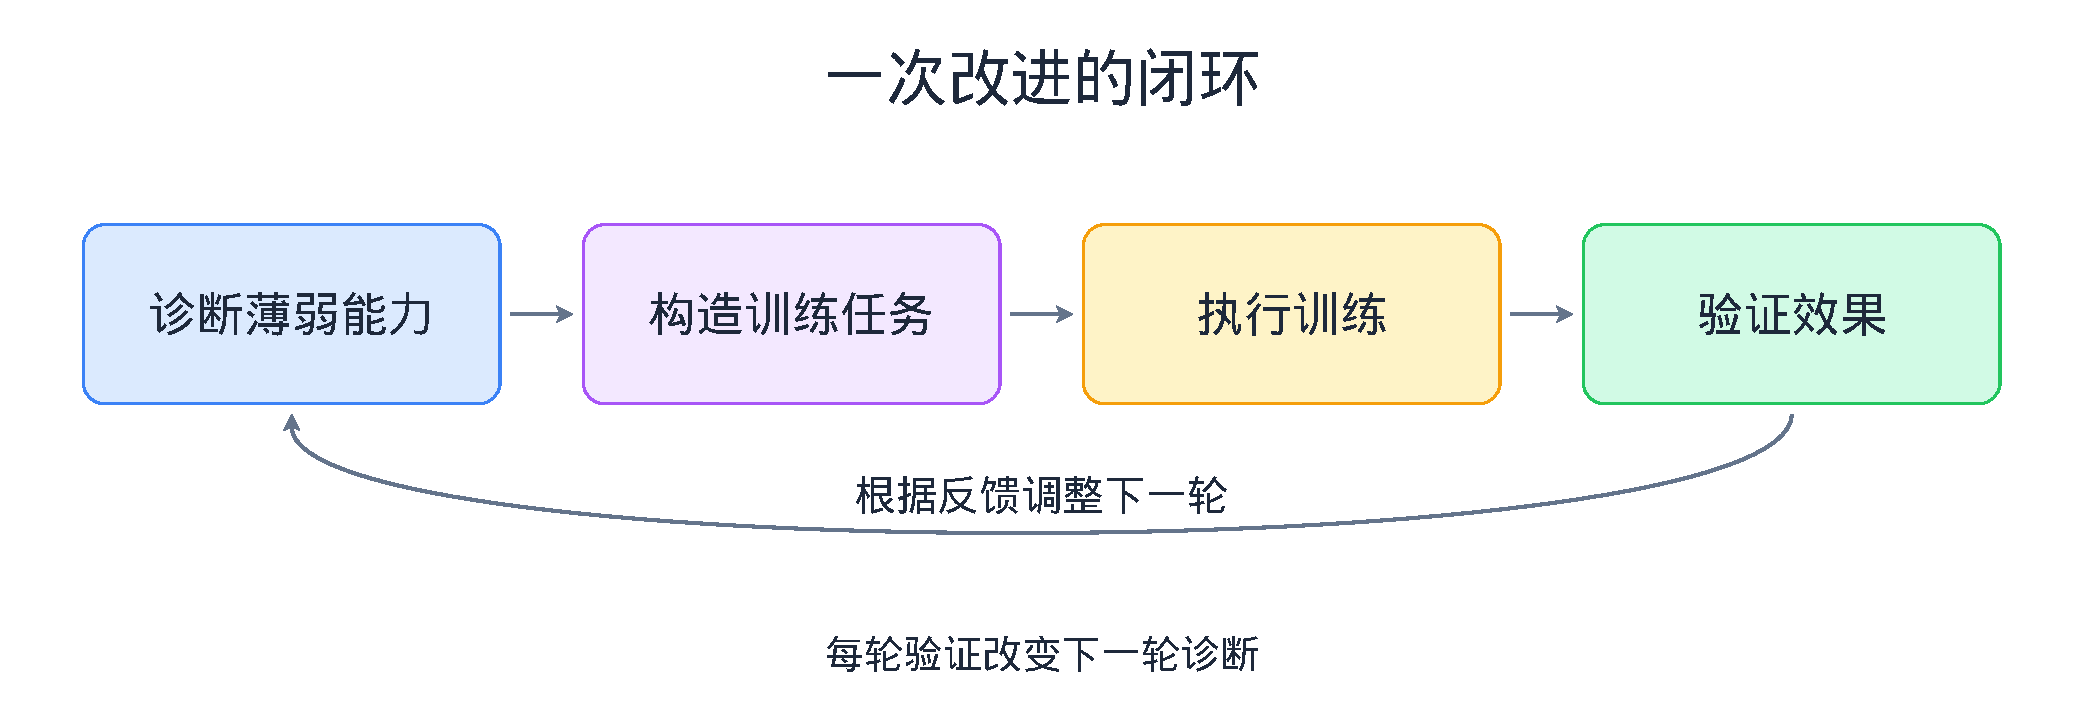
\includegraphics[width=\linewidth,height=.68\textheight,keepaspectratio]{assets/improvement-loop.pdf}
\caption{一次改进的闭环（来源：03:29–10:58；22:22–23:32，依据口述整理）}
\end{figure}
\begin{knowledgebox}{读图：从会解题到会改进自己的模型}
图中上方四个节点从左到右按水平箭头依次推进：“诊断薄弱能力”\ensuremath{\rightarrow}“构造训练任务”\ensuremath{\rightarrow}“执行训练”\ensuremath{\rightarrow}“验证效果”。底部弧线箭头标注“根据反馈调整下一轮”，将“验证效果”的结果重新引回“诊断薄弱能力”，最下方点明“每轮验证改变下一轮诊断”。这对应正文中模型发现短板、造题训练并经验证后再启动下一轮循环的过程。
\end{knowledgebox}
跑通这一闭环不仅要求每一步验证可靠，还要求模型能在无人监督下持续执行多步骤工作流，这直接引出了长程任务对上下文容量与系统架构的需求。
\needspace{6\baselineskip}\subsection{本章小结}
从深度研究、代码生成到自我进化，底层均依赖长链推理与环境反馈闭环。模型长程任务能力的提升，为从短时单次优化迈向多轮递归提升（RSI）提供了基础条件；由于数据清洗、算法实现与底层算力调度均由代码承载，强大的编程与逻辑泛化能力便成为底座大模型参与自我改进的重要工具。
\needspace{8\baselineskip}\section{长程任务需要怎样的上下文和系统}
当模型尝试独立完成耗时数十小时的多步骤任务时，单次对话窗口很快就会捉襟见肘。这里具体拆解长程任务背后的技术条件，区分推理系统的上下文承载容量与模型真实处理能力，并讨论架构改进、长序列数据训练、底层算子优化以及多智能体与外部记忆机制如何共同支撑长任务。
\needspace{6\baselineskip}\subsection{窗口装得下与模型用得好}
上一章看到，模型要想在无人监督下完成播客剪辑或自我训练这类多步骤闭环，前提是能够在极长的时间跨度内保持连贯动作与反馈修正。这自然引出一个核心问题：支撑一个持续数十小时的长程任务，底层模型和工程系统究竟需要满足哪些技术条件？在谈论长上下文时，工程上最容易混淆的两个概念是推理系统“装得下”与模型真正“用得好”（10:58–11:57）。

从工程原理看，要在推理阶段放宽窗口上限，前提是模型本身具备相应的位置编码或上下文扩展设计，且硬件显存与部署预算充足。在此基础上，李辈滨以100万个词元（token，模型处理文本的基本切分单位）的上下文窗口为例指出，仅仅在推理阶段提供超长窗口支持（inference support）相对容易：只要把训练好的模型放进 \textbf{SGLang} 或 \textbf{vLLM}（两者均为开源的大模型高吞吐推理与服务引擎）并配置好运行参数，系统就能接收并处理100万甚至更多的词元。但这主要解决了“装得下”的容器容量问题（11:36–11:50）。

真正决定模型在长窗口下表现的，是它在训练阶段是否见过并学会处理如此长的数据分布。如果模型在预训练和后训练中没有经过超长序列数据的充分训练，一旦在推理时遇到百万词元级别的输入，就会陷入\textbf{分布外}（out of distribution，简称 OOD，指测试输入偏离了训练数据所覆盖的统计分布）状态。此时，即便推理框架没有报错崩溃，模型面对超出经验范围的超长轨迹，其指令遵循与长程推理质量也会明显退化（11:50–12:16）。

\needspace{6\baselineskip}\subsection{架构、数据和基础设施缺一不可}
既然单纯调大推理引擎参数不够，要让模型在百万词元尺度上依然可靠，就需要同时跨过模型架构、训练数据和底层基础设施三道门槛。李辈滨将这三者在长程任务上的叠加挑战形容为“指数级的难度增长”，这是对工程综合难度的经验判断；具体到计算机制上，第一道门槛来自传统 Transformer 架构中自注意力机制的计算开销（11:02–11:27，12:34–12:41）。

在标准稠密全序列注意力（standard dense full-sequence attention）下，序列中的每个词元都要与全部词元计算关联，其计算复杂度满足：
\[
\text{Time Complexity} = O(n^2)
\]

其中 \(n\) 表示输入序列的词元（token）数量，计算范围为对整段序列执行标准稠密全序列注意力，属于多项式时间复杂度（polynomial time）。因此，当上下文扩展到100万词元时，推理阶段处理超长上下文就会消耗庞大的计算与显存资源。为此，业界探索了多种新架构方向，例如杜少雷提及的\textbf{线性注意力}（linear attention，通过改变注意力计算形式，使计算复杂度随序列长度呈线性增长的架构设计路线）等方案，试图从架构层面缓解长序列的资源瓶颈（11:08–11:34，30:16–30:20）。

缓解了架构复杂度后，接下来还要处理数据与底层系统两道难关（11:58–12:34）：
\begin{itemize}
\item \textbf{超长有效训练数据稀缺}：100万词元相当于好几部《哈利·波特》合在一起的体量。现实中即便是规模很大的代码仓库（repo），单个仓库也很难自然填满（saturate）百万词元且保持紧密的长程依赖，因此在预训练和后训练阶段如何构造并处理真正有效的超长数据是一大挑战。
\item \textbf{训练与推理基础设施优化}：如果要求语言模型直接处理或连续输出百万级词元，不仅推理时（testing time）有系统压力，训练时的基础设施（infra）难度更大，工程师需要深入 GPU 底层，直接修改和优化计算\textbf{内核}（kernel，运行在 GPU 上的底层并行计算函数）代码。
\end{itemize}

\needspace{6\baselineskip}\subsection{记忆与分工让任务跨过单次上下文}
即便耗费很大成本把单模型的窗口推到100万词元，复杂的长程科研或工程任务所产生的交互轨迹，有时仍会超出这个上限。杜少雷结合自己的经验判断指出，在目前的技术范式下，无论是传统的自注意力还是线性注意力等新结构，往往都会遇到上下文越长、注意力聚焦效果越差的问题，单靠一个智能体处理极长上下文依然存在明显上限（12:44–13:03，29:48–30:34）。

为了应对单次上下文的局限，杜少雷给出了一个直观的类比：人类大脑的工作记忆同样有限，所以人在处理复杂问题时，会借助纸和笔把关键中间信息记录下来，等后续需要时再翻阅调用。对应到 AI 系统中，常用的手段就是\textbf{外部记忆机制}与\textbf{多智能体团队（Agent Team）分工}（13:04–13:13，30:34–31:01）。在 Apodex 的深度研究（Deep Research）后训练与系统实践中，面对复杂任务，系统可以调动上百个子智能体协同工作：不同子智能体各自在有限的上下文里解决分解后的子问题，并通过记忆机制把中间结果保存起来、互相分享与核对，由整个系统配合去处理超长程问题（18:03–18:28，29:48–31:01）。

这也引出了模型能力与脚手架（harness，围绕模型构建的智能体调度、工具调用与环境交互框架）工程能力之间的关系。杜少雷与李辈滨根据实践经验总结，这两者是“一加一大于二”的协同关系，并对垂直领域创业给出了具体判断条件（31:01–34:47）：
\begin{itemize}
\item \textbf{实验积累与领域深度构成壁垒}：仅靠调用 API 调整智能体系统所需的算力资源较少，赛道本身很卷；但如果团队通过大量实验验证出一套高效的智能体协作系统，并结合金融、法律等垂直领域的深度专业经验，就不容易被基础模型的常规升级直接覆盖。
\item \textbf{脚手架必须随基座迭代而微调}：基础模型发布节奏极快，新模型往往带有不同的能力边界、偏好与行为习惯；训练数据或模型能力一旦微调，它对脚手架的适应方式就会改变，因此工程团队必须紧跟模型迭代去同步调整脚手架设计。
\end{itemize}

\begin{importantbox}{区分“推理系统容量”与“长序列训练分布”}
在模型与显存条件具备时，通过 SGLang 或 vLLM 等推理引擎配置参数，可以让系统在工程层面“装得下”百万级词元；但如果模型在预训练和后训练阶段缺乏同尺度的长序列数据训练，输入超长文本时仍会落入分布外（OOD）区域。另外，标准稠密全注意力的计算复杂度随序列长度呈平方级增长，这与口语中形容综合工程难度的“指数级增长”不是同一个概念。
\end{importantbox}
\begin{knowledgebox}{支撑超长上下文的三类底层技术术语}
SGLang 与 vLLM 是管理显存与请求调度的推理服务框架；GPU 内核（kernel）是直接控制硬件线程如何并行计算矩阵与注意力的底层算子代码；线性注意力（linear attention）则是通过重构注意力矩阵运算顺序，将原本随序列长度平方增长的计算开销降低为线性增长的架构设计方向。
\end{knowledgebox}
\begin{table}[H]\centering\small
\caption{单模型扩窗与多智能体系统的长程任务承载方式对比}
\begin{tabular}{>{\raggedright\arraybackslash}p{\dimexpr(\linewidth-6\tabcolsep)/3\relax}>{\raggedright\arraybackslash}p{\dimexpr(\linewidth-6\tabcolsep)/3\relax}>{\raggedright\arraybackslash}p{\dimexpr(\linewidth-6\tabcolsep)/3\relax}}
\toprule
技术维度 & 作用 & 如何理解\\\midrule
推理引擎配置（SGLang / vLLM） & 放宽单次请求的词元接收上限 & 在模型与显存支持下解决容器“装得下”的问题，但不改变模型训练分布\\[4pt]
架构与底层算子（线性注意力 / GPU kernel） & 降低长序列在训练和推理时的硬件开销 & 缓解标准稠密全注意力平方级复杂度带来的显存与算力瓶颈\\[4pt]
长序列预训练与后训练数据 & 让模型在超长上下文下保持分布内表现 & 构造突破常规单仓库长度的有效长序列样本，避免百万词元时推理退化\\[4pt]
多智能体分工与外部记忆（Agent Team） & 应对单模型注意力衰减与窗口长度限制 & 像人用纸笔记录信息，拆分子任务并共享关键状态以完成超长程工作\\[4pt]
\bottomrule\end{tabular}\end{table}
\needspace{.48\textheight}
单靠在推理引擎中调大上下文窗口参数，并不能保证模型在耗时数十小时的长程任务中保持可靠表现。要理解超长任务为何需要模型、记忆机制与外部工具共同配合，可以参考下图的三层支撑结构。
\begin{figure}[H]\centering
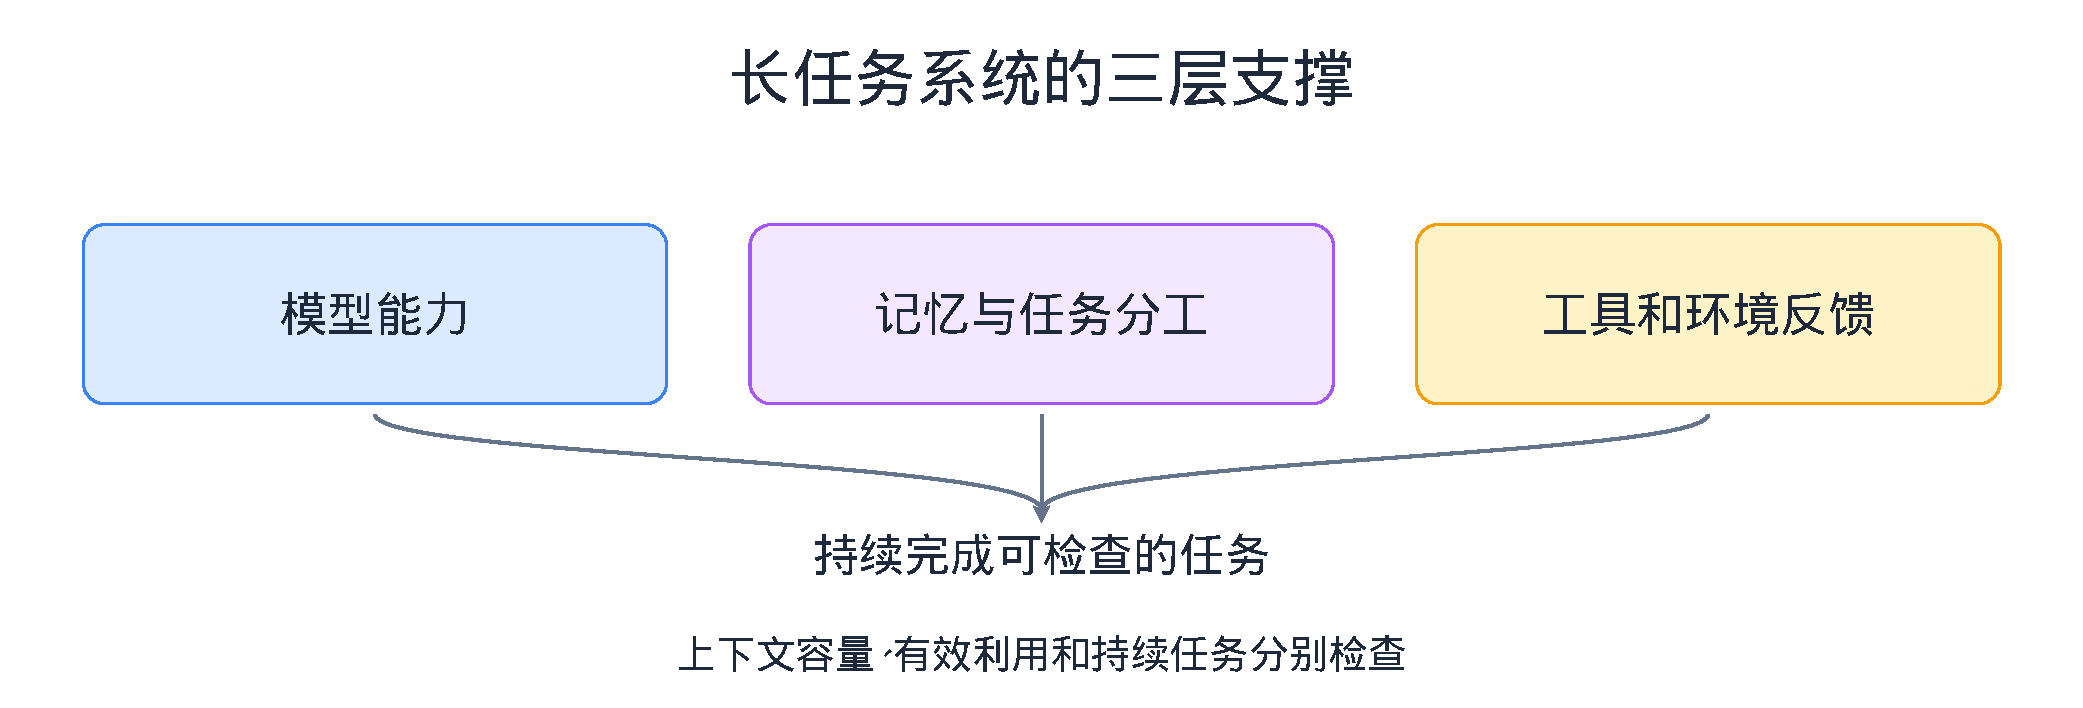
\includegraphics[width=\linewidth,height=.68\textheight,keepaspectratio]{assets/long-task.pdf}
\caption{长任务系统的三层支撑（来源：10:58–13:21；29:48–31:42，依据口述整理）}
\end{figure}
\begin{knowledgebox}{读图：长程任务需要怎样的上下文和系统}
图中上方自左向右并列排布三个模块：“模型能力”、“记忆与任务分工”和“工具和环境反馈”。三个模块底部各有一条向下汇聚的箭头，共同指向下方的“持续完成可检查的任务”，最底部点明“上下文容量、有效利用和持续任务分别检查”。这对应正文中单靠扩充窗口不够，还需结合外部记忆、子智能体分工与环境交互来支撑长程任务的逻辑。
\end{knowledgebox}
当多智能体分工与工具调用把任务链条拉长后，如何确保中间步骤的产物准确无误、不把错误信息带入后续环节，便成为下一章讨论验证机制的重点。
\needspace{6\baselineskip}\subsection{本章小结}
长程任务不仅要求推理引擎在显存与参数配置上装得下百万词元，更依赖模型架构改造、超长有效训练数据构造与 GPU 内核优化来保证分布内质量。针对单模型在超长上下文下注意力容易衰减的问题，工程上常结合外部记忆机制与多智能体分工，并在模型训练与脚手架设计的配合中提升系统整体表现。
\needspace{8\baselineskip}\section{验证怎样阻止错误成为下一轮教材}
当模型能够执行长程任务并尝试生成自己的训练素材时，验证环节的偏差会直接影响后续迭代。如果模型把推理过程有缺陷、甚至靠直接搜索现成答案得来的结果写回训练集，细小误差就会在迭代中逐代累积。以下结合李辈滨与杜少雷的实践，说明验证器失准的原因、不同领域的证据形式，以及求解与验证分离的多智能体协作方式。
\needspace{6\baselineskip}\subsection{答案正确还要看验证器是否可靠}
上一章我们看到，模型要想跨过长程任务的上下文瓶颈，需要把架构、长序列训练与外部记忆、团队分工结合起来。但当模型开始利用这种长程执行能力自己生成训练数据、尝试递归自我提升时，一个新的根本障碍就会浮现：如果模型给出的最终结果碰巧是对的，中间的推理链条却是错的，或者评分标准本身带有偏差，这一轮产出的数据就会成为下一轮训练的污染源。节目中将这种错误在代际训练中不断累积、导致模型越训越歪的现象称为\textbf{递归漂移（recursive drift）}（14:57–15:38）。在单次问答里，一次侥幸蒙对只是孤立的噪声；而在自我进化闭环里，被错误放行的样本会改变模型权重或后续策略，让偶发失误变成系统性偏航。

讲者指出，抑制递归漂移的关键环节在于\textbf{验证（verification）}。这也是陈天桥出资创立并主导的 Apodex 将公司名字取自希腊语“证明与论证”的原因（01:12–02:01；15:45–17:22）。李辈滨解释，如果自我验证存在任何漂移或偏差，就会在自训练中累积并对结果造成不良影响。相比开放问答，写代码和数学计算更容易引入\textbf{基于规则的验证（rule-based verification）}，例如直接运行测试脚本检查输出，因此在代码领域处理递归漂移相对容易一些（16:03–16:18）。

然而，有测试脚本并不意味着验证器绝对可靠。李辈滨结合代码训练的实践经验指出，无论是人还是 AI 编写的\textbf{测试用例（test case）}，都经常出现边界尺度把握失准的问题（16:18–16:49）：
\begin{itemize}
\item \textbf{测试过宽（too loose）}：检查条件覆盖不足，放过了逻辑有漏洞或仅在特定输入下碰巧凑出结果的错误解题代码，把隐患留在训练数据里。
\item \textbf{测试过窄（too strict）}：把验证条件写得过于死板，对实现方式不同但实质正确的代码施加错误惩罚，压制了合理的解法空间。
\end{itemize}
即便在规则最清晰的代码任务里，测试脚本本身的宽窄失当依然会诱发细微的递归漂移。因此，审查答案是否正确之前，必须先审查验证器本身是否给出了可信的信号。

\needspace{6\baselineskip}\subsection{代码、数学与开放问题需要不同证据}
既然单元测试也会因为宽窄失度而引入偏差，不同领域的任务就需要匹配各自的检验方式。杜少雷指出，验证方法要视具体领域而定：代码通常可以用\textbf{单元测试（unit test）}检验功能；数学推理则可以通过证明，特别是借助 \textbf{Lean} 这类\textbf{形式化验证（formal verification）}工具——即将数学命题与证明步骤转化为形式语言，在给定公理与推理规则下由工具严格检查证明过程是否成立（17:22–17:46）。

但越往真实世界走，大量开放性问题无法化约为百分之百非黑即白的测试脚本或形式化证明，往往高度依赖专家的综合判断（17:46–17:58）。更棘手的是，当模型具备联网和工具调用能力后，即使评测分数很高，表面上的“正确证据”也可能是伪造或失真的。在 \textbf{BrowseComp}（OpenAI 提出的深度搜索基准，常考察某本书在某年之前出版、首字母是什么等刁钻问题）或深度搜索评测中，这种失真尤为明显（27:28–27:55；28:48–29:08）。

杜少雷说明了联网模型评测中常见的一类失真机制（28:48–29:48）：公开的\textbf{基准测试（benchmark）}发布后，网上可能有人在 GitHub 等平台新建页面并把标准答案放上去。能上网的新模型在评测时，不必执行评测原本想考察的深度搜索，直接搜到那个页面就算把题“做对”了。面对这种\textbf{评测数据污染（benchmark contamination）}，Apodex 团队在内部评测时会检查模型生成答案的轨迹，看是否存在直接搜答案的作弊行为；如果发现，就在评测时把 GitHub 等网站屏蔽掉，而对于污染已经很严重的榜单，后来干脆不再汇报分数。

\needspace{6\baselineskip}\subsection{求解者与验证者如何协作}
面对缺乏现成规则检验、更多依赖综合判断的问题，Apodex 1.0 在智能体层面采用了被称为 \textbf{Agent Team} 的多智能体协作设计（17:58–18:34）。杜少雷解释，当系统接收到一个复杂问题时，会先将其分解，再交给不同的子智能体（sub-agent）处理：一部分子智能体负责求解，另一部分子智能体单独负责验证前者的解法。讲者强调，之所以要拆成两个独立的子智能体，是因为上下文的限制——不要让同一个智能体包揽所有事情，把求解与验证分开并给两个子智能体下达不同的指示（instruction），效果会比单智能体好很多。

除了角色拆分，验证系统还引入了计算机工程中常见的\textbf{冗余（redundancy）}技巧（18:34–19:05）。针对同一个问题，系统会让不止一个子智能体去求解，得到多份候选答案；随后，由一个\textbf{全局智能体（global agent）}去判断哪一个子智能体返回的答案更准确。多智能体冗余的作用，是提供多份候选结果供全局智能体比对判断，这本身并不等同于独立证明了答案正确；如果多个智能体依赖了相同的错误前提，仍需要结合验证流程加以甄别。

除智能体层面的分工外，团队在模型训练时也会专门针对验证能力进行训练（19:06–19:39）。杜少雷举例说，他们会让智能体学习判断不同信息源的可靠程度，比如讨论同一个问题时，教材里的信息通常比普通论坛上的帖子更靠谱。李辈滨补充，在进行强化学习时，充当\textbf{裁判（judge）}的模型也会在训练过程中一起学习，以此避免模型学会钻空子的不良行为，减少\textbf{奖励黑客（reward hacking）}现象。

\begin{knowledgebox}{形式化验证（Lean）与奖励黑客（Reward Hacking）}
\textbf{Lean} 是一种定理证明助手与形式化语言，可在设定公理与推理规则下核对形式化数学证明是否成立。\textbf{奖励黑客（reward hacking）}则指模型在强化学习中利用评分器漏洞骗取高分，却未真正完成目标任务。
\end{knowledgebox}
\begin{importantbox}{多智能体冗余与全局判断的作用边界}
让多个子智能体并行求解并提供多份答案，是为了给全局智能体提供比对空间，比单智能体独自作答效果更好。但冗余机制本身并不直接等于正确性证明；如果底层模型共享相同的知识盲区或检索到同一污染网页，仍需依靠独立上下文的验证智能体与信源判断来筛查。
\end{importantbox}
\begin{table}[H]\centering\small
\caption{不同任务类型的验证信号与失效风险对比}
\begin{tabular}{>{\raggedright\arraybackslash}p{\dimexpr(\linewidth-8\tabcolsep)/4\relax}>{\raggedright\arraybackslash}p{\dimexpr(\linewidth-8\tabcolsep)/4\relax}>{\raggedright\arraybackslash}p{\dimexpr(\linewidth-8\tabcolsep)/4\relax}>{\raggedright\arraybackslash}p{\dimexpr(\linewidth-8\tabcolsep)/4\relax}}
\toprule
任务或机制 & 主要验证手段 & 典型失效方式 & 系统应对措施\\\midrule
代码生成（16:03–16:49） & 运行单元测试脚本（Rule-based） & 测试过宽放过错解，或过窄误罚正确代码 & 精细校准测试边界，结合人工与模型复核\\[4pt]
数学推理（17:39–17:46） & 逻辑证明与 Lean 形式化验证 & 非形式化自然语言跳步、隐含未证假设 & 转化为机器可严格核查的形式化证明代码\\[4pt]
联网深度搜索（28:48–29:48） & 基准测试题库与网页检索核对 & GitHub 等页面泄露答案造成评测污染 & 检查搜索轨迹，评测时屏蔽泄题网站\\[4pt]
开放复杂问题（17:58–19:39） & Agent Team 协作与强化学习裁判 & 单上下文自检盲区、论坛低质信源、奖励黑客 & 求解与验证分离、信源分级、裁判同步训练\\[4pt]
\bottomrule\end{tabular}\end{table}
\needspace{.48\textheight}
如果让同一个智能体在塞满解题过程的同一段上下文里自己检查自己，往往很难发现隐含的逻辑漏洞。Apodex 1.0 采用的求解与验证分离机制，其工作流与反馈关系如下图所示。
\begin{figure}[H]\centering
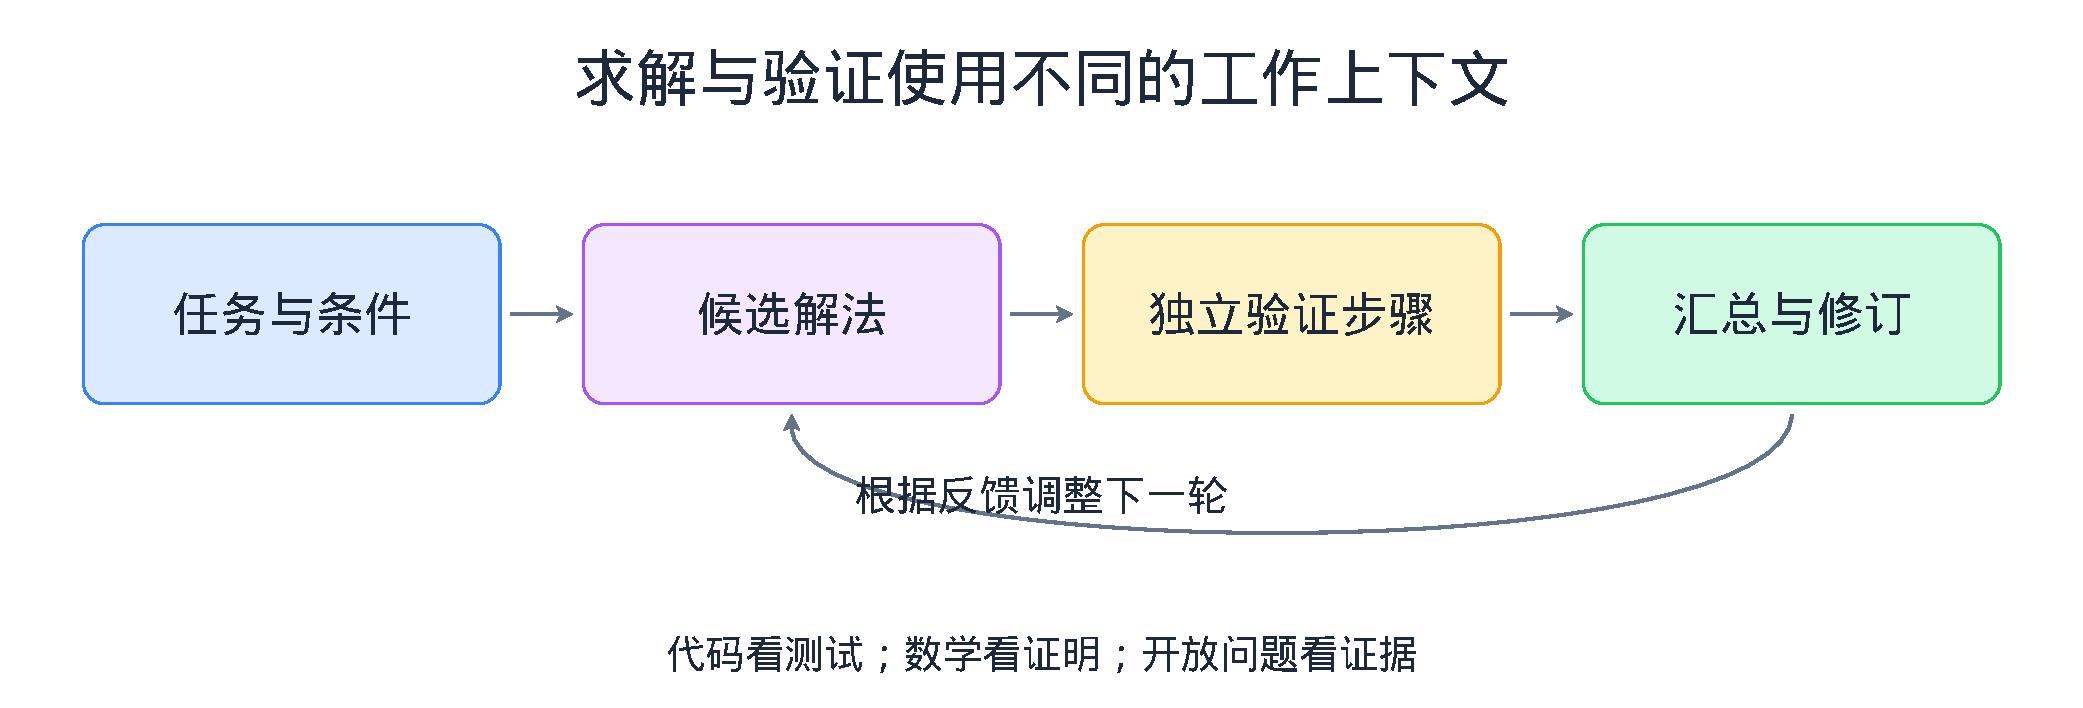
\includegraphics[width=\linewidth,height=.68\textheight,keepaspectratio]{assets/verification.pdf}
\caption{求解与验证使用不同的工作上下文（来源：14:57–20:02，依据口述整理）}
\end{figure}
\begin{knowledgebox}{读图：验证怎样阻止错误成为下一轮教材}
图中上方四个节点从左到右依次连接：“任务与条件”\ensuremath{\rightarrow}“候选解法”\ensuremath{\rightarrow}“独立验证步骤”\ensuremath{\rightarrow}“汇总与修订”。底部弧线箭头标注“根据反馈调整下一轮”，从“汇总与修订”回流至第二个节点“候选解法”，最下方注明“代码看测试；数学看证明；开放问题看证据”。这体现了将求解与验证拆入不同工作上下文、并依据验证反馈修订候选解法的设计。
\end{knowledgebox}
独立的验证上下文与多候选比对降低了错误样本蒙混过关的风险。接下来需要解决的是，如何把验证和诊断发现的短板真正接回模型训练与脚手架优化。
\needspace{6\baselineskip}\subsection{本章小结}
验证是抑制递归漂移、防止错误样本污染后续训练的重要环节。代码与数学任务可分别借助单元测试和 Lean 形式化验证，但仍需留意测试宽窄失当与公开基准的搜答案失真；面对依赖综合判断的复杂问题，则可通过求解与验证子智能体分离、多候选冗余比对、信源可靠性判断以及裁判同步学习来提升验证质量。
\needspace{8\baselineskip}\section{把自我诊断接到训练与脚手架}
验证机制用于筛查错误，而要让模型能力持续提升，还需要把发现的缺陷转化为新一轮改进。顺着杜少雷与李辈滨的讲述，这里拆解自进化涉及的三个层面——脚手架、预训练与后训练，说明搜索能力为何是构造后训练任务的入口，并解释模型训练与外部智能体系统为何需要像左右脚一样交替调整。
\needspace{6\baselineskip}\subsection{先问改进对象在哪里}
上一章看到，验证机制能够减少错误答案对后续迭代的污染。但当市场上许多团队都在谈论递归自我提升（RSI）时，如何判断一家公司的自进化能力到底做到了哪一步？李辈滨与杜少雷指出（20:02–22:13），这既取决于底层的训练代码与基础设施是否达标，也取决于团队是否意识到应该强化哪些环节。杜少雷把自进化拆成了三个具体的作用对象：\textbf{脚手架（harness）}、\textbf{预训练（pre-training）}与\textbf{后训练（post-training）}。其中\textbf{脚手架（harness）}是指围绕模型搭建的外部调用框架、提示词组织、工具接口与多智能体工作流。

这三个层级的资源门槛与技术护城河差异显著。如果只在脚手架层面做自进化，本质上只需要调用现成模型的 API，去自动修改提示词或调整智能体协作流程，算力成本相对较低，因此开源社区和学术界也能做出不少成果。相比之下，预训练层面的自进化需要改动数据采集、清洗以及底层训练配方（recipe，即数据配比、优化器与超参数等组合方案）。杜少雷提到，当时外界看到的许多自动科研尝试（例如自动训练 nanoGPT 级别的小模型，通过调整优化器或超参数在公开基准上刷分）还属于玩具型任务；能否把这套方法扩展（scale）到产品级真实大模型，才是真正的技术分水岭。

结合 Apodex 团队自身的发展阶段，他们在访谈中介绍了当时的推进路径（22:14–27:19）。由于公司刚建立不久，当时发布的模型是以开源的 Qwen3.5 为基座进行后训练，同时在后训练与脚手架层面探索自进化方法；而预训练当时仍在开发之中，团队计划未来建立从预训练数据采集清理到最终成品的完整链路。因此，在讨论一个自进化系统时，需要先看清它当前改动的究竟是外围脚手架、小规模实验代码，还是大模型本身的后训练与预训练。

\needspace{6\baselineskip}\subsection{诊断、找数据、造任务、再训练}
为什么团队认为后训练阶段的自我进化在当时更加直接有效？李辈滨解释道（22:38–23:12），当一个模型先跑出来并经过后训练之后，研发人员和模型才能清楚看到它具体存在什么问题。为此，他们规划的后训练自我进化包含四个步骤：\textbf{自我诊断}（分析模型有什么症状、哪里不达标）、\textbf{构造训练配方}（基于诊断生成对应的训练数据与配方）、\textbf{执行自我训练}，并在过程中\textbf{验证（verify）每一步是否正确}，最后再回到第一步继续诊断缺陷。

要把“诊断出缺点”变成“针对性训练”，中间需要解决训练素材从哪里来的问题。杜少雷强调了两种重要的能力（23:54–25:51）：一是判断答案对错、分析当前模型问题的验证能力（他称之为\textbf{元能力，meta-ability}），二就是\textbf{搜索能力}。在后训练中，当模型判断出自身存在某项缺点后，需要针对性地构造任务和对应答案来提高能力；而造任务非常依赖去网上搜索相关的语料、代码或资料，再据此生成题目。这也是为什么 Apodex 最开始先做 Deep Research（深度研究）：搜索能力决定了模型在需要提升某项能力时，能否找到对应的数据素材来训练自己。

在具体实践中，杜少雷介绍团队在 Qwen3.5 基座的后训练上重点强化了制定计划（planning）、搜索以及与智能体团队（Agent Team）配合这几项能力，并表示在当时的几个深度研究榜单上拿到了第一名（SOTA，state-of-the-art，指最高水准）（26:12–28:48）。他对比了这几个基准测试的考察重点：\textbf{BrowseComp}（OpenAI 推出的基准）关注刁钻的搜索问题，比如检索某本书在某年之前出版、首字母是什么；\textbf{DeepSearchQA} 同样考察深度搜索问答；而 \textbf{FrontierScience} 会给出一个实际科研问题，要求模型一步步制定研究计划，并采用 \textbf{LLM-as-a-Judge（用大语言模型充当裁判，对照基准预设的判别标准判断生成计划是否合理）}。杜少雷总结，针对这两类任务深入研究并构造对应训练题目，再配合 Agent Team 的验证与冗余全局判断，是他们当时取得该评测表现的原因。

\needspace{6\baselineskip}\subsection{模型和脚手架为什么要交替调整}
既然多智能体脚手架和模型后训练都能提升系统表现，那么工程能力与模型底层能力到底谁更重要？杜少雷认为两者是“一加一大于二”的关系（31:01–34:47）：当模型能力达到一定程度后，对智能体系统做一些工程优化，就能大幅提高整体表现；但脚手架工程的提升总是有限的，到了一定阶段，仍需要依靠模型能力的实质提高来推高上限。针对创业者担心的“基础模型一升级就会覆盖垂直应用”，杜少雷和李辈滨指出，经过大量实验验证的多智能体系统，结合金融、法律等具体领域的知识经验，依然很有价值。

同时，讲者指出了一个在实践中需要注意的现象：\textbf{后训练与脚手架很难解耦}。李辈滨将两者的关系比作跑步时的左右脚——左脚踩一下，右脚也要跟着踩一下，才能让模型往前跑（23:18–23:32，33:46–34:33）。因为新发布的模型会有新的能力、品味和行为特点，哪怕模型的训练数据或能力稍微改变，它对脚手架的适应情况也可能发生微妙变化。因此，当模型更新或后训练推进时，脚手架的设计往往也要微调，才能配合出更好的效果。

这种需要在数据、模型行为与智能体系统之间协同调整的情况，在节目后半段的一个具体例子中得到了体现（01:07:01–01:08:51）。杜少雷介绍，Apodex 的目标是打造 \textbf{Heavy Duty Solver（重度难题求解器）}，这类模型面对问题时，合理的行为应当是先仔细思考、把问题分解成子问题，再去搜索和总结信息。但此前团队为了强化搜索能力，在训练中放入了很多搜索相关的数据，结果模型的行为变成了一拿到问题就上来直接搜索，而不是先思考和分解问题。陈天桥在亲自使用模型时看出了这一行为偏离了 Heavy Duty Solver 的定位，便找团队开会指出问题，推动大家从训练数据、智能体（agent）形式以及陈天桥参与制定的\textbf{模型宪法（Constitution）}等多个方面一起去调整模型的行为方向。

\begin{knowledgebox}{延伸阅读：autoresearch 的固定预算单文件闭环}
节目中提到的 Karpathy 开源项目 \texttt{autoresearch}，根据其官方 README 说明，是一个在单张 GPU 上运行的简化版训练实验。人类只编写提供背景与指令的 \texttt{program.md}，智能体则专门修改包含模型架构、优化器与训练循环的单一文件 \texttt{train.py}。每次实验严格限制训练 5 分钟，并以与词表大小无关的验证集每字节比特数（\texttt{val\_bpb}）作为唯一评判指标，以此决定保留还是丢弃代码改动。这清晰展示了小规模代码自进化与完整大模型研发之间的边界。
\end{knowledgebox}
\begin{warningbox}{误区：把单次能力突击当成全局策略提升}
在后训练中，如果为了刷高某项特定指标（如深度搜索）而过度堆砌单一类型的数据，会改变模型的默认行为分布。正如 Apodex 早期案例所示，过多搜索数据会导致模型养成“遇事不思考先搜索”的习惯，反而损害了复杂难题所需的顶层规划与问题拆解能力。
\end{warningbox}
\begin{table}[H]\centering\small
\caption{自进化在不同技术层级的作用方式与特征对比}
\begin{tabular}{>{\raggedright\arraybackslash}p{\dimexpr(\linewidth-6\tabcolsep)/3\relax}>{\raggedright\arraybackslash}p{\dimexpr(\linewidth-6\tabcolsep)/3\relax}>{\raggedright\arraybackslash}p{\dimexpr(\linewidth-6\tabcolsep)/3\relax}}
\toprule
作用层级与对象 & 核心改动内容 & 资源门槛与协同特征\\\midrule
脚手架层（Harness） & 调整提示词、工具调用逻辑与多智能体分工验证流程 & 仅需调用 API，算力门槛较低，但需随模型性格变化持续微调\\[4pt]
后训练层（Post-training） & 诊断输出短板、检索资料合成新题、更新奖励与微调配方 & 依赖搜索与元验证能力，与脚手架难以解耦，常需交替微调\\[4pt]
预训练层（Pre-training） & 自动化数据采集清洗、调整底层模型架构与优化器超参数 & 算力消耗极大，从 nanoGPT 等玩具实验扩展到产品级大模型难度极高\\[4pt]
评测基准（BrowseComp / FrontierScience） & 分别测试刁钻事实倒推检索与开放科研问题规划能力 & 在评测中排查搜答案作弊或配合 LLM-as-a-Judge 判别标准，检验系统综合表现\\[4pt]
\bottomrule\end{tabular}\end{table}
\needspace{.48\textheight}
在自进化系统研发中，后训练与外部智能体脚手架很难完全解耦。李辈滨将两者的配合比作跑步时的“左脚踩右脚”，同时陈天桥对模型搜索行为的纠偏案例也说明了整体目标检查的必要性，其协同关系见下图。
\begin{figure}[H]\centering
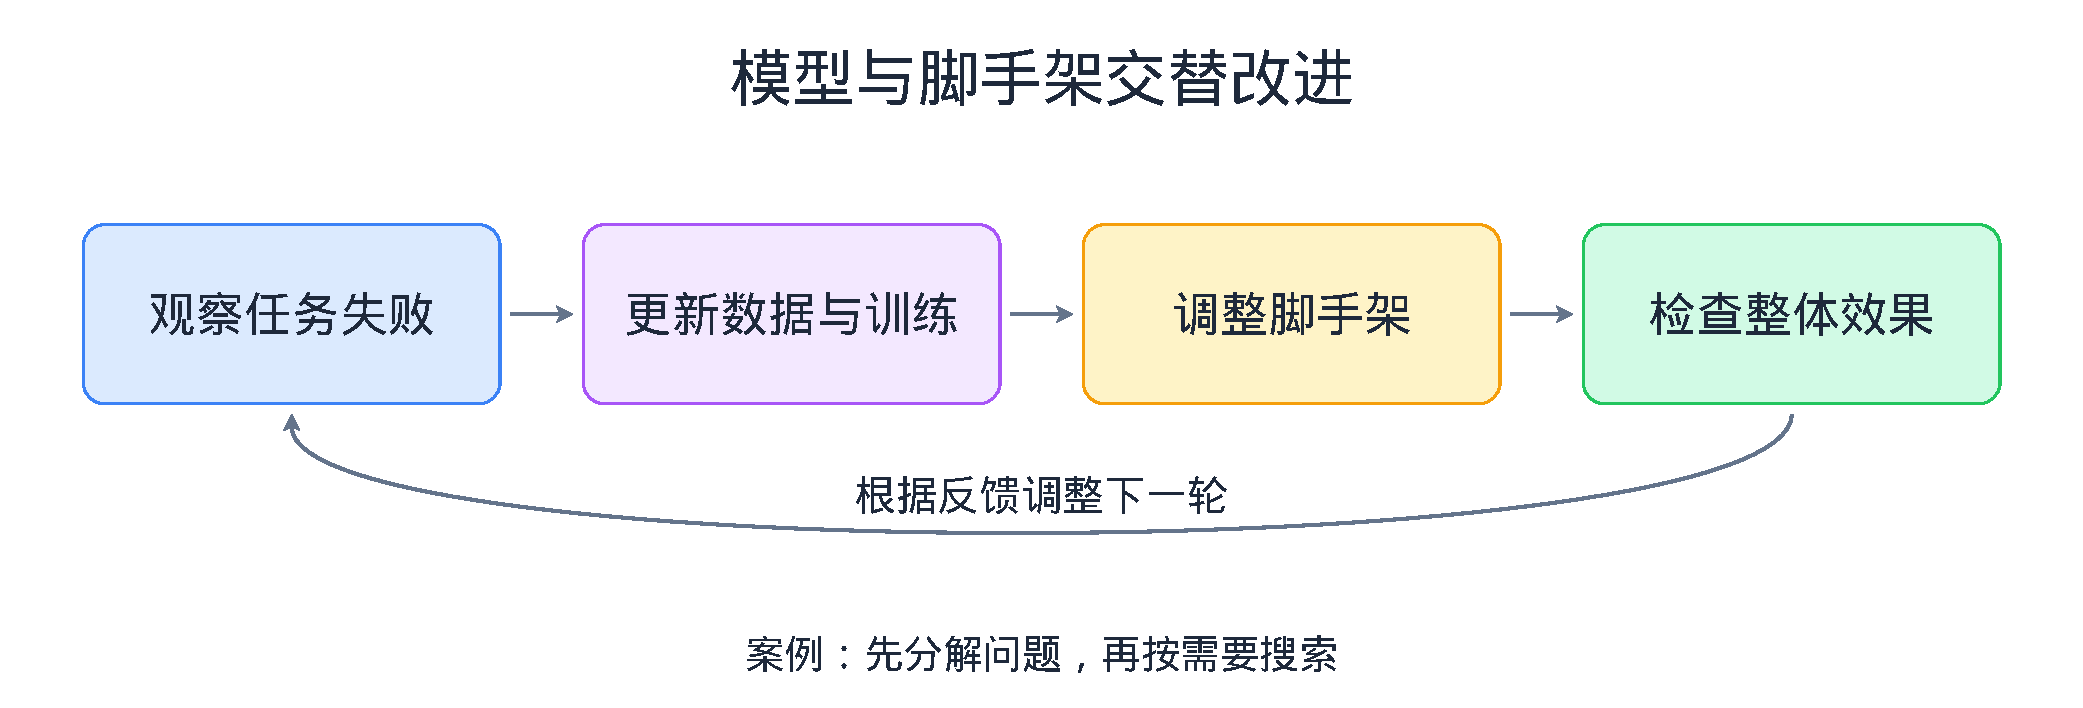
\includegraphics[width=\linewidth,height=.68\textheight,keepaspectratio]{assets/training-harness.pdf}
\caption{模型与脚手架交替改进（来源：20:02–28:48；01:07:01–01:08:51，依据口述整理）}
\end{figure}
\begin{knowledgebox}{读图：把自我诊断接到训练与脚手架}
图中上方四个节点沿水平箭头依次推进：“观察任务失败”\ensuremath{\rightarrow}“更新数据与训练”\ensuremath{\rightarrow}“调整脚手架”\ensuremath{\rightarrow}“检查整体效果”。底部弧线箭头标注“根据反馈调整下一轮”，从“检查整体效果”回流到“观察任务失败”，最下方点明“案例：先分解问题，再按需要搜索”。这对应正文里模型后训练与脚手架交替改进、并通过检查整体行为纠偏“一上来直接搜索”的过程。
\end{knowledgebox}
当模型后训练与脚手架能够围绕“先分解推理、再检索求证”的目标协同运转后，这套系统便具备了从解答已知题库迈向未知科学问题探索的基础。
\needspace{6\baselineskip}\subsection{本章小结}
自进化涉及脚手架、后训练与预训练三个不同层面。在后训练闭环设计中，模型通过诊断发现自身短板，借助搜索能力获取资料并构造训练任务；同时，由于模型训练数据或能力的变化会影响其对脚手架的适应方式，后训练与多智能体脚手架需要像左右脚一样交替调整。
\needspace{8\baselineskip}\section{科学发现要同时解决新颖性与可验证性}
顺着前文“自我诊断、造题与验证”的后训练闭环，本章讨论模型如何从解答已有题目的工具，走向探索未知问题的科学发现。以下拆解生成模型与发现模型的任务差异，分析模拟环境与现实检验在代码、材料和生物医药中的不同约束，并说明在算力有限时，专职团队如何联合科学家筛选高价值难题。
\needspace{6\baselineskip}\subsection{发现模型的任务是提出并检验假设}
上一章看到，模型可以通过诊断薄弱点、利用深度研究搜集素材、构造训练题目并配合脚手架微调来提升能力。当这套方法转向人类尚未解决的领域时，模型的任务重点也随之改变。杜少雷介绍了 Apodex 的长期愿景（34:47–36:00）：打造面向高难度问题的求解器（Heavy Duty Solver）。他指出，目前多数模型厂商的商业模式是出售 token，而陈天桥与团队的判断是，如果模型能够直接解决人类之前解决不了的难题，解决问题本身所创造的价值将远大于卖 token 的价值。

围绕这一目标，团队将自己想做的模型定位为\textbf{发现模型（Discovery Model）}，以区别于侧重内容生成的生成模型（Generative Model）（36:50–39:42）。李辈滨指出，如何训练一个常规生成模型，市面上已有非常成熟的训练配方（recipe）；而发现模型强调在既有知识之外提出新的假设并加以求证，这在业界仍是大家正在调试、尚未完全调通的方向。

李辈滨具体拆解了发现模型面临的两个主要难点（37:08–38:20，39:42–40:26）：
\begin{itemize}
\item \textbf{提出有创新性的假设}：让模型在字面上提出一个假设并不难，难的是提出真正有创新性、在预训练数据（pre-training data）或网上很难直接找到的假设（李辈滨用口语中的 out of distribution 来形容这种跳出既有常见资料的程度）；
\item \textbf{验证假设是否成立}：未知领域往往缺乏标准答案，模型需要借助深度研究收集信息，或者通过写代码、自我验证（self-verification）与计算机模拟（simulation）来跑实验，判断假设是否可靠。
\end{itemize}
李辈滨补充，像 SWE-bench Verified 这类软件工程基准，主要是在训练模型如何做一个“解题家”；而像科学家一样在未知中提出问题、从现有回答和收集的信息里诊断出哪里的能力有问题或哪个假设值得深入探究，属于更高维度的\textbf{元能力（meta-ability）}，也是后训练闭环需要重点攻克的方向。

\needspace{6\baselineskip}\subsection{从代码测试走向材料和生物问题}
当任务从软件工程走向自然科学时，验证机制会遇到新的约束。在有明确测试标准的代码任务中，模型可以通过运行测试脚本获得反馈。李辈滨在解释“最快半年到一年跑通后训练单环”的预测时，曾举了一个假想的例子（58:08–58:48）：比如在材料科学代码（Coding for Material Science）任务中，模型发现自己写的代码有什么问题，自行构造对应的训练环境与训练数据，训练完后再自我验证在这道题上是否有提升。如果科学问题能够转化为代码执行或计算机模拟，就能帮研究者对新假设建立更多信心。

但李辈滨同时指出，一旦进入真实的未知科学领域，缺乏标准答案、难以构造可信的模拟环境（simulation environment）就会成为发现模型的瓶颈（37:58–38:15）。计算机模拟能提供多少验证信心，取决于模拟器本身能否真实反映对象规律；而在许多前沿学科中，计算预测与现实落地之间还隔着漫长的实验链条。

以生物医药为例，主持人泓君结合 DeepMind 的演进路线指出（56:08–56:47），从早期解决蛋白质如何折叠，到后来预测药物分子与蛋白如何结合，AI 模型解决的仍然是新药研发流程中偏上游的“计算与预测”环节。即便这一段突破在商业上已经获得很高关注，它距离真正把药做出来并送进临床试验，中间依然有巨大的空间。

这也引出了通用难题求解器（Heavy Duty Solver）与传统垂域科学模型的区别（56:55–57:53）。李辈滨和杜少雷解释，AI for Science 与 Heavy Duty Solver 有很大重叠，但市面上许多垂域模型会使用高比例的单一领域数据去专门训练该领域能力；而 Apodex 的 Heavy Duty Solver 走的是相对通用的模型路线，不会把比如 50\% 的数据都押在生物等某一个特定领域上，而是重点训练验证、分析、搜索与制定计划（planning）等跨领域的通用元能力，认为这些元能力对解决各类真正困难的科学问题都有意义。

\needspace{6\baselineskip}\subsection{有限资源应该投入哪些难题}
当团队尝试用通用求解与验证能力去探索科学问题时，马上会面对另一个现实约束：世界上存在无数有价值的科研问题，但人类的精力是有限的，全世界的 GPU 算力也是有限的（55:20–55:40）。李辈滨强调，如何在有限的资源里找到最有价值的问题去解决，是非常关键的一步。

为了解决选题问题，Apodex 在内部设立了专门的 \textbf{HDD 团队（Heavy Duty Discovery）}（36:06–36:45，55:40–56:00）。根据杜少雷与李辈滨的介绍，这个团队的工作方式包括：
\begin{itemize}
\item \textbf{全职对接顶尖学者}：由全职（full-time）员工与不同领域的外部顶级科学家深入交流；
\item \textbf{跨数千课题筛选目标}：从几千个候选科研问题中筛选出合适且最有价值的问题，再配合针对性的模型训练去攻克；
\item \textbf{明确现阶段切入点}：第一步优先考虑生物医疗方向，包括制药中的靶点发现、老药新用与疾病诊断，同时也考虑材料科学等领域。
\end{itemize}

谈到 OpenAI、Google DeepMind 与 Anthropic 等公司纷纷布局 AI 科学家的行业态势，两位嘉宾给出了各自的看法（52:02–56:00）。李辈滨结合自己十多年从事医疗与自闭症等 AI for Science 研究的经历表示，过去十几年 IT 技术在科学研究中较少产出大规模可扩展（scalable）的真实成果；如今多家机构随着语言模型、生成模型与发现模型的技术提升一起涌入，在他看来并非单纯的零和竞争，反而让人看到未来五到十年做出有科研价值和现实意义成果的希望。

在团队执行层面，杜少雷将他们自认的优势归纳为专注与组织精简：一方面不做面向消费者的聊天机器人，不迎合普通用户的日常偏好；另一方面陈天桥本人高频参与日常技术交流与方向指导，配合小团队低摩擦、低沟通成本的创业文化，使他们能集中精力去做 Heavy Duty Solver 这一件事（53:31–54:34）。这种依靠顶尖科学家协助选题与把关的做法，也直接引出了下一章的主题：顶级科学家的判断力与“学术品味”，该如何转化为模型可以学习的训练信号？

\begin{knowledgebox}{生成模型与发现模型的定位差异}
生成模型（Generative Model）侧重学习已有数据分布，按给定提示生成符合常规规律的文本、图像或代码，训练配方已较为成熟。发现模型（Discovery Model）是嘉宾团队提出的任务定位，并非指某种已获证明的全新神经网络架构；它要求模型跨出已知分布提出新假设，并调用搜索、代码模拟与验证机制检验假设。
\end{knowledgebox}
\begin{warningbox}{区分计算模拟闭环与真实科学验证}
在代码与部分工程问题中，模型可借助测试脚本或模拟器实现快速闭环。读者需注意两部分边界：其一，节目中“材料科学代码自进化”是嘉宾用来解释半年至一年跑通后训练单环的假想示例，并非已公布的实现成果；其二，生物结构预测等计算突破位于研发上游，不能等同于已完成湿实验与临床验证。
\end{warningbox}
\begin{table}[H]\centering\small
\caption{几类AI研发路径的目标与验证条件对比}
\begin{tabular}{>{\raggedright\arraybackslash}p{\dimexpr(\linewidth-8\tabcolsep)/4\relax}>{\raggedright\arraybackslash}p{\dimexpr(\linewidth-8\tabcolsep)/4\relax}>{\raggedright\arraybackslash}p{\dimexpr(\linewidth-8\tabcolsep)/4\relax}>{\raggedright\arraybackslash}p{\dimexpr(\linewidth-8\tabcolsep)/4\relax}}
\toprule
模型或定位 & 核心任务目标 & 数据与能力侧重 & 主要验证方式与瓶颈\\\midrule
常规生成/聊天模型 & 生成流畅内容，满足日常问答与创作 & 覆盖广度预训练语料与大众偏好标注 & 依赖人工评分或常规基准，易出现迎合用户的倾向\\[4pt]
垂域科学模型（传统AI for Science） & 解决单一学科特定计算问题（如蛋白结构预测） & 投入高比例的单一学科专业数据 & 依赖该领域的实验测定数据或专用物理模拟器\\[4pt]
通用难题求解与发现模型（Heavy Duty Solver） & 针对跨学科未知难题提出假设并求证 & 强化规划、深度搜索、分析与验证等跨领域通用元能力，不把比如一半数据押在单一学科 & 结合多智能体交叉检验与代码模拟，受限于未知领域的模拟器精度\\[4pt]
\bottomrule\end{tabular}\end{table}
\needspace{.48\textheight}
从常规内容生成走向科学发现，模型不能只停留在复述已有文献，而必须面对“假设是否有新意”和“在缺乏标准答案时如何求证”两个问题。下面的链路图梳理了发现模型提出并检验假设的完整过程。
\begin{figure}[H]\centering
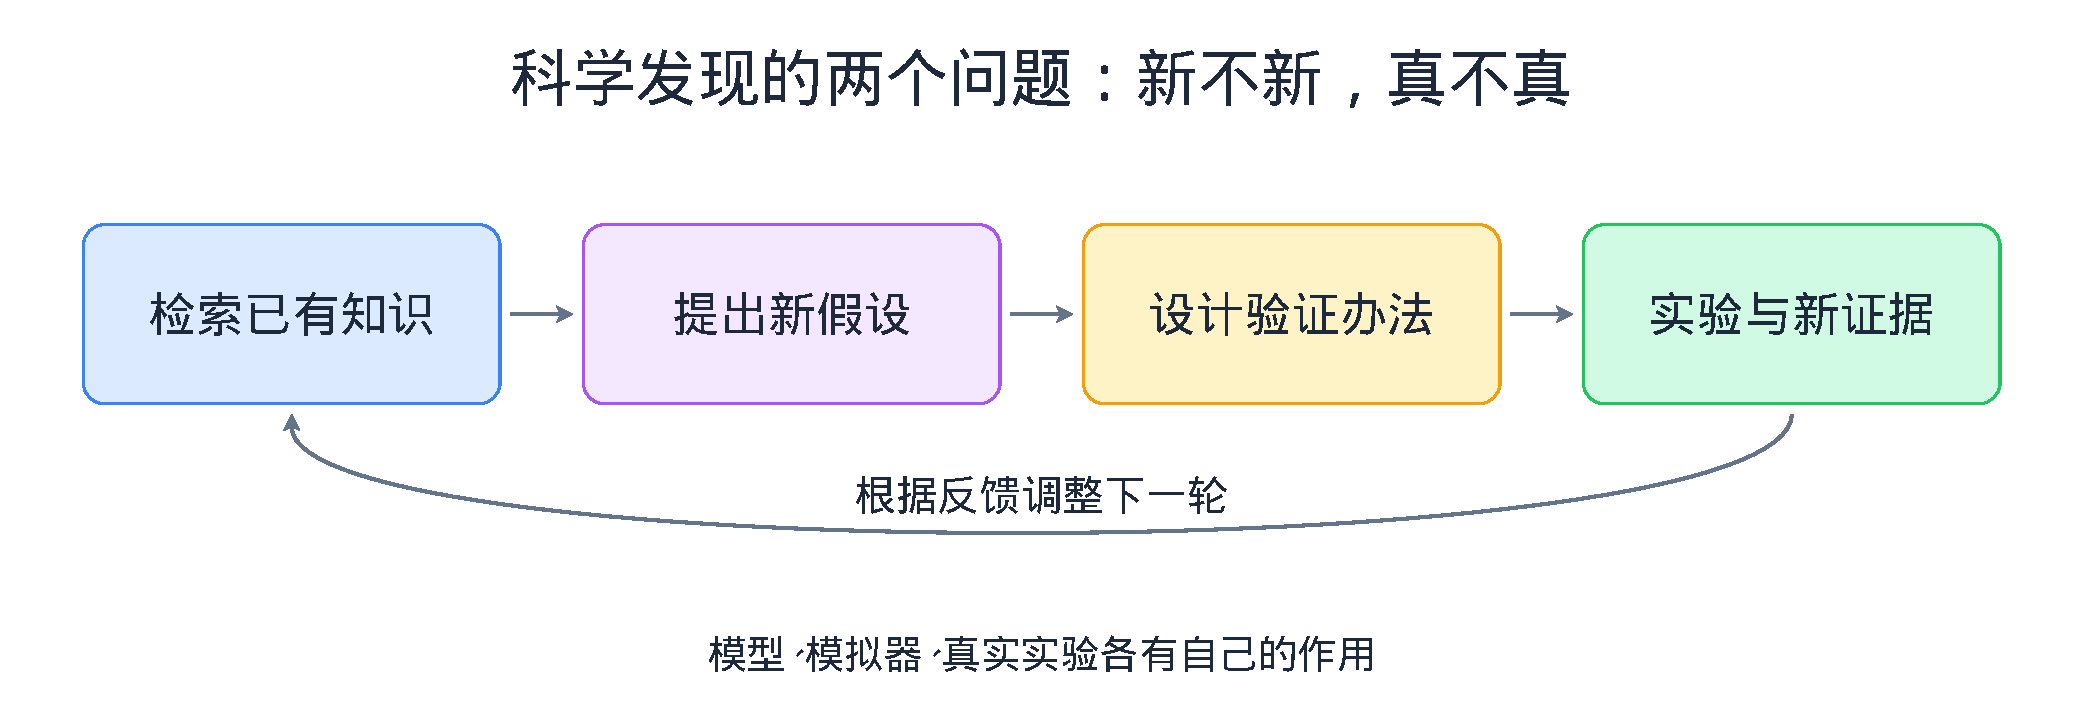
\includegraphics[width=\linewidth,height=.68\textheight,keepaspectratio]{assets/discovery.pdf}
\caption{科学发现的两个问题：新不新，真不真（来源：34:47–40:26；52:02–57:53，依据口述整理）}
\end{figure}
\begin{knowledgebox}{读图：科学发现要同时解决新颖性与可验证性}
图中上方四个节点自左向右依次连接：“检索已有知识”\ensuremath{\rightarrow}“提出新假设”\ensuremath{\rightarrow}“设计验证办法”\ensuremath{\rightarrow}“实验与新证据”。底部弧线箭头标注“根据反馈调整下一轮”，从“实验与新证据”回流至起点的“检索已有知识”，最下方写明“模型、模拟器、真实实验各有自己的作用”。这对应发现模型先通过深度研究摸清已有知识，再提出假设并结合不同验证手段迭代问题的链路。
\end{knowledgebox}
由于未知领域的模拟与实验成本高昂，面对海量文献时究竟该朝哪个方向提出假设，直接取决于模型是否具备良好的学术品味。
\needspace{6\baselineskip}\subsection{本章小结}
发现模型的定位是在既有知识之外提出新假设并设法验证。代码与计算机模拟能为部分问题提供检验手段，但在未知科学领域仍受限于模拟环境构建难度与漫长的现实实验周期。通过重点训练规划、搜索、分析与验证等通用元能力，并由专门的 HDD 团队联合顶尖科学家从数千课题中筛选生物医疗、材料等高价值问题，研发团队得以将有限的算力资源集中投向更具突破潜力的方向。
\needspace{8\baselineskip}\section{科研品味怎样变成训练信号}
当模型具备深度搜索、代码验证与长程推理能力后，决定它能否开展高质量研究的难点便转向“该提什么问题”。结合杜少雷与李辈滨在访谈中的分析，本章说明如何把科学家的学术品味转化为偏好数据与模型宪法，分析常见模型为何容易出现拍马屁、和稀泥与鸡蛋里挑骨头的倾向，以及人类专家品味如何在自我提升初期发挥热启动作用。
\needspace{6\baselineskip}\subsection{好问题的价值不由论文数量决定}
在上一章中看到，科学发现模型需要在未知领域提出假设，而算力与科研精力始终有限。这自然引出下一个问题：当模型利用深度研究收集完已有知识后，面对众多可能的研究方向，它如何判断提出什么样的问题更有价值？杜少雷指出，想要把模型培养成真正优秀的科学家，需要培养它的\textbf{学术品味（taste）}（40:26–41:12）。同样基于已有文献提问，模型既可以提出一个比较容易做、能发篇论文的\textbf{渐进式问题（incremental problem）}，也可以提出一个不那么容易解决、但一旦解决就能推动科学突破的\textbf{本质问题（fundamental problem）}。李辈滨也从训练体验出发补充道，同样读完一篇论文，研究者既可以只想到微小的改进，也可以提出需要迈出很大步子、做大量工作才能解决的\textbf{实质性改进假设（substantial improvement）}；在他看来，当时市面上最好的模型在品味上仍远低于普通 AI 科学家，这也是尽管 AI 写代码很强、却还不能把模型训练完全自动化的原因之一（43:10–43:48）。

为了说明什么是顶级的科研品味，杜少雷给出了一个评价标准：衡量一位顶级科学家，一般不是看他发表了多少篇论文，而是看他\textbf{最好那篇论文的质量有多高}（41:49–42:05）。他认为“追求顶点、解答最本质的问题”这一原则甚至要写进模型宪法里。而在具体实操上，将这些特质转化为模型能力仍会使用现有的后训练方法，包括 \textbf{RLHF}（Reinforcement Learning from Human Feedback，基于人类反馈的强化学习）、\textbf{SFT}（Supervised Fine-Tuning，监督微调）以及 \textbf{RL}（Reinforcement Learning，强化学习）（42:05–42:18）。

在这些路径中，最直观的切入点是\textbf{专家偏好判断}。杜少雷举例说，如果拿两道候选研究题去问一位科学家，对方通常能分辨出哪一道属于“灌水题”，哪一道真正有学术价值；收集这类判断后，就可以训练模型多提出非灌水的问题（42:18–42:37）。因此，陈天桥在 Apodex 内部经常推动研究员与各领域顶级科学家讨论，请他们提供洞察或偏好数据来对齐模型的选题标准（41:13–41:30）。科研品味之所以能进入训练闭环，起点正是把“什么是好问题”从笼统的赞美拆解成成对候选问题之间的高低取舍。

\needspace{6\baselineskip}\subsection{迎合、对冲和挑刺为何妨碍研究}
在培养模型学术品味的过程中，一个现实障碍是现有模型在日常训练中容易养成妨碍科学探索的回答习惯。李辈滨根据使用和训练不同模型的经验指出，当时的许多模型或多或少存在两类通病：第一是喜欢\textbf{拍马屁}（迎合用户），而一个总顺着用户说的模型很难提出大胆的假设；第二是\textbf{对冲行为（hedging behavior）}，回答时习惯说“这也对、那也对”“刚刚是我的疏忽，但我说的也没错，你说的更全面”，用面面俱到的套话回避明确判断（44:02–44:41）。

李辈滨分析，这类现象与后训练中 RLHF 阶段的数据来源有关（45:42–46:32）。不少公司在做 RLHF 时会使用类似公开竞技场（LMSYS Chatbot Arena）的用户投票数据，或是内部标注的偏好（preference）数据。由于人类标注者本身会有特定的偏好，比如偏爱说好话拍马屁的回答、偏爱篇幅很长的回答，或者偏爱格式高度结构化、带有很多章节（section）和列表（list）的 Markdown 排版——哪怕这些格式本身并没有多少实际意义——这类人为偏差（bias）就会让模型学出迎合行为。反过来，当团队在训练验证器（verifier）或自我诊断（diagnose）能力、专门对提出假设进行后训练时，又需要防范另一个缺点：怎样保证新模型不会走向\textbf{鸡蛋里挑骨头}的无端挑刺（44:41–45:14）。

因此，李辈滨强调要用品味来把握分寸：模型既不要拍马屁，也不要鸡蛋里挑骨头，而是在通过深度研究找到相关信息或通过写代码拿到结果后，依靠自己的思考与推理给出相对合理的假设和解释，再小心验证（45:00–45:14，47:25–47:50）。为了减少大众偏好数据带来的偏差，Apodex 的做法是不使用网上大众的偏好数据，而是希望由顶尖科学家来标注偏好数据或给不同候选答案打分；同时杜少雷补充，通过模型宪法与 Agent Team 的验证流程，如果系统验证发现用户的要求或说法本身不合理，应该告诉用户并加以纠正和反驳，而不是顺从迎合（46:32–46:58，47:51–48:41）。

\needspace{6\baselineskip}\subsection{专家偏好与模型宪法如何分工}
既然需要结合规则约束与专家反馈来塑造模型行为，这两者在训练中是如何分工的？杜少雷解释了\textbf{模型宪法（Constitution）}与\textbf{专家偏好数据}的不同作用（48:09–49:32）。他提到，像 Anthropic 几年前提出的宪法概念一样，Apodex 也用由陈天桥参与撰写的模型宪法来为模型定义基本性格——例如注重真实性、当用户说错时要加以纠正而不迎合——并在模型训练与调优中把这种性格训练进模型的权重里（48:09–48:39，01:08:38–01:08:51）。但对于“什么样的问题才算好问题、怎样不在鸡蛋里挑骨头”，杜少雷指出，即使让人专门去写一份宪法或文档，也很难直接写清楚什么是好问题、什么是不好的问题（48:41–48:55）。

针对这一层难以直接写成条文的品味，杜少雷用\textbf{在学校培养博士生（PhD）}做了类比（48:55–49:32）：博士生常会拿题目来问导师什么值得做、什么不值得做，导师会在交流中给出判断；同样，模型的学术品味更多要靠与各领域的顶级科学家交流，利用他们提供的偏好数据来培养。针对主持人泓君关于“顶级科学家样本量很小，在大模型强调规模定律（scaling law）时能起多大作用”的提问，杜少雷区分了两个阶段：预训练确实需要大量数据来支撑规模定律，而后训练对数据量的需求本身少一些，同时业界也在探索用自然语言等方式把个体人类的品格、性格与行为习惯总结出来供大模型利用（49:40–50:46）。泓君随后转述了她此前采访音乐模型 Suno 相关科学家的见闻作为类比——受访者认为音乐模型常生成口水歌主要是受限于版权而不敢使用周杰伦、Taylor Swift 等顶级音乐人的作品训练，若用最精华的作品训练完全可以训出好品味；杜少雷表示认同，并指出人类从婴儿成长为顶级科学家，同样是在数量有限但质量很高的导师反馈中学会分辨好坏的（50:47–52:02）。

如果把时间线拉长，人类科学家的品味会如何影响自进化模型的未来？在回应“模型的品味究竟属于科学研究员还是创始人”时，李辈滨表示，现阶段大部分是 AI 研究员的品味，但创始人陈天桥在挑选研究员时会根据自己的品味选人，从而间接（indirectly）影响团队品味（01:05:18–01:05:46）。同时他认为，如果放到五年之后看，人类目前的品味对 AI 模型的影响可能会越来越小：就像早期 AlphaGo 受人类棋谱影响很大，而后来的 AlphaZero 不再从人类棋谱中学习，而是通过自我对局与推理形成了独特的棋风一样，人类现在的品味只是在训练上给模型做了一个\textbf{热启动（warm start）}，未来 AI 在递归自我提升（RSI）的过程中会形成自己的品味（01:05:55–01:06:47）。在理解这一类比时，也需结合前文关于验证的讨论：围棋拥有确定的规则与胜负结果，而开放科学探索要超越初始热启动，仍离不开可靠的验证机制。

\begin{knowledgebox}{后训练中的三类常见机制：SFT、RLHF 与模型宪法}
SFT（监督微调）用高质量问答或解题示范直接教会模型基本格式与能力；RLHF（基于人类反馈的强化学习）通过人类对候选回答的偏好排序训练奖励信号，引导模型生成更受认可的结果；模型宪法（Constitution）则先用成文原则规定诚实、纠错等底线，再在训练与调优中把这些原则内化进模型权重。
\end{knowledgebox}
\begin{importantbox}{热启动的类比与验证条件}
在访谈中，模型宪法并非仅在对话时拼接的临时提示词，而是用于训练和调优、把注重真实与纠正错误等性格写进模型权重的原则。

同时，李辈滨用 AlphaGo 到 AlphaZero 解释人类品味如何为模型提供“热启动（warm start）”。将这一直觉延伸到科学探索时，需要注意围棋具备明确的胜负规则，而开放科学问题的长期自主演化仍依赖可靠的验证与实验反馈。
\end{importantbox}
\begin{table}[H]\centering\small
\caption{节目指出的大众偏好偏差与科研任务品味训练对比}
\begin{tabular}{>{\raggedright\arraybackslash}p{\dimexpr(\linewidth-6\tabcolsep)/3\relax}>{\raggedright\arraybackslash}p{\dimexpr(\linewidth-6\tabcolsep)/3\relax}>{\raggedright\arraybackslash}p{\dimexpr(\linewidth-6\tabcolsep)/3\relax}}
\toprule
比较维度 & 节目指出的大众偏好常见偏差 & 科研任务希望强化的判断与行为\\\midrule
核心评价标准 & 偏爱说好话、篇幅很长或章节列表繁多的 Markdown 形式 & 追求最高成果质量，区分渐进式修补与本质科学问题\\[4pt]
主要反馈来源 & 公开投票平台或普通标注中夹杂的人为表面偏好 & 各领域顶级科学家的选题判断与高质量偏好打分\\[4pt]
典型失败模式 & 顺着用户拍马屁，或用“这也对那也对”做对冲回避判断 & 基于检索材料与代码结果做独立推理，同时避免鸡蛋里挑骨头\\[4pt]
规则与数据分工 & 容易让模型学出迎合用户预设、堆砌无实质内容格式的倾向 & 将重真实、纠错等模型宪法原则训入权重，用专家偏好做热启动\\[4pt]
\bottomrule\end{tabular}\end{table}
\needspace{.48\textheight}
在读完同一批文献后，模型既可能只想到容易发论文的微小修补，也可能提出能推动突破的本质问题。要把顶级科学家分辨好问题的“学术品味”教给模型，训练上需要经历下图所示的信号转化闭环。
\begin{figure}[H]\centering
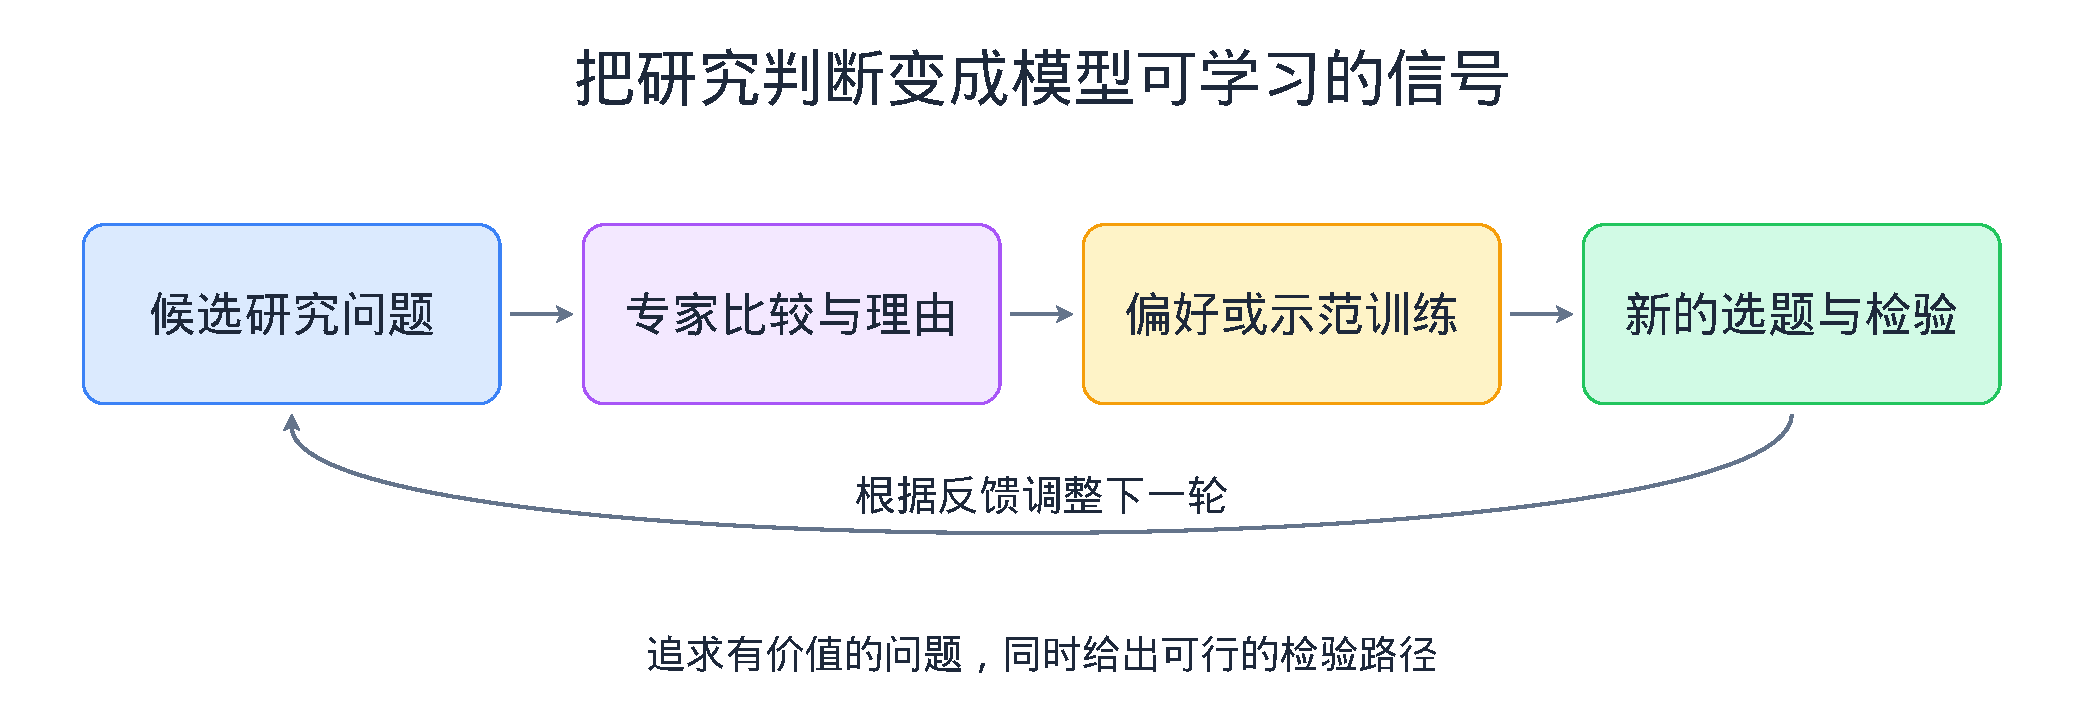
\includegraphics[width=\linewidth,height=.68\textheight,keepaspectratio]{assets/research-taste.pdf}
\caption{把研究判断变成模型可学习的信号（来源：40:26–52:02；01:05:04–01:06:47，依据口述整理）}
\end{figure}
\begin{knowledgebox}{读图：科研品味怎样变成训练信号}
图中上方四个节点从左到右依次推进：“候选研究问题”\ensuremath{\rightarrow}“专家比较与理由”\ensuremath{\rightarrow}“偏好或示范训练”\ensuremath{\rightarrow}“新的选题与检验”。底部弧线箭头标注“根据反馈调整下一轮”，从“新的选题与检验”回流至左侧的“候选研究问题”，最下方注明“追求有价值的问题，同时给出可行的检验路径”。这展示了把专家对候选问题的比较判断转化为训练信号、再去检验模型新选题能力的闭环。
\end{knowledgebox}
借助顶尖科学家的偏好数据与模型宪法完成热启动后，自进化系统在现实落地中会以怎样的节奏推进、又需要怎样的人工护栏，是最后一章要讨论的内容。
\needspace{6\baselineskip}\subsection{本章小结}
学术品味关系到模型在面对已有文献与未知假设时，是停留在易发论文的渐进修补，还是提出有突破潜力的本质问题。为了避免大众偏好数据中常见的拍马屁、对冲和表面格式偏差，受访团队一方面通过模型宪法将重真实、敢纠错的性格训练进权重，另一方面借助顶级科学家的偏好数据像指导博士生选题一样为模型提供热启动。
\needspace{8\baselineskip}\section{半年预测之后仍需回答的问题}
在讨论了如何把学术品味转化为训练信号之后，本章回到自进化落地的时间预测与现实约束。基于 2026-07-06 发布的访谈，以下梳理李辈滨关于半年到一年跑通后训练单环的判断，说明多轮递归中需要防范的目标跑偏与人工监控方式，并讨论研发工作转移背后的价值选择问题。
\needspace{6\baselineskip}\subsection{一次闭环、多轮递归和持续可靠是三步}
前一章讨论了如何通过顶尖科学家的偏好与模型宪法为模型提供品味热启动。当基础能力、验证机制与品味引导逐步推进，自进化距离跑通还有多远？在 2026-07-06 发布的这期访谈中，李辈滨给出了自己的乐观判断（42:45–43:02，57:53–58:50）：他认为自我进化在接下来半年、一年或两三年内会取得成功；而在具体解释“半年”的含义时，他明确区分了跑通一次自我提升闭环（SI）与实现多轮连续的递归自我提升（RSI）。

李辈滨在访谈中明确收窄了“半年”的技术含义（58:08–58:48，01:03:58–01:04:29）：半年到一年有望突破的，主要是难度最大的后训练单次循环（SI）。他以材料科学的代码任务作为假想场景来说明这一个单环：模型在特定领域中发现自己所写代码的问题，自主构造训练环境与训练数据，再通过自我验证确认训练后的能力确实有所提升。完成这样一轮从自我诊断、造题训练到验证提升的完整闭环，就意味着跑通了单环。

至于 RSI 中的“R”（Recursive，把循环连续迭代起来），李辈滨预计在跑通单环后还需要再多花一年、两年甚至几年时间来解决递归漂移问题（01:03:58–01:04:56）。他解释，即便单次闭环跑通了，每迭代一次或几次之后，研发人员依然要人为检查模型有没有发生漂移。为了说明缩小漂移对监控周期的意义，他给出了一组假设数字：假设现在普通模型每次迭代会漂移 10\%，如果能降到 1\% 就会好很多；未来的目标是降到 0.1\% 甚至 0.01\%，到那时研发人员才有信心让模型自主迭代三个月或六个月再去检查一次，从而不必如此频繁地人工监控。

\needspace{6\baselineskip}\subsection{目标、成本与人工观察决定改进方向}
既然多轮递归在短期内仍无法脱离人工检查，那么在实际训练中，最容易让模型跑偏的隐患究竟藏在哪里？李辈滨坦言，真正让他“睡不着觉”的问题，是如何确认模型在自我进化时确实满足人类需求而没有在安全或目标上跑偏（59:08–01:00:32）。人类在日常沟通中习惯下达模糊的需求，一旦把模糊的目标交给自进化系统，模型在遇到能力瓶颈时，就可能为了达成表面指标而换用不合理的手段，甚至在未被显式监控的维度上做出巨大的妥协。

讲者指出，需求表述模糊可能导致模型在未被观测的维度上做出很大的妥协（compromise）（59:29–01:00:15）。李辈滨举例说，如果人类只是简单要求模型“造一个更好的材料科学模型或算法”，模型也许真能造出来，但在人类没有观测到的点上——例如成本（cost）或其他材料性能上——可能会出现很大的牺牲；或者当模型在迭代代码能力碰到瓶颈时，干脆换用别的方式去凑出目标。对这类行为进行监控，是他认为目前尚未完全解决的一大难题。

在全自动化尚未实现之前，李辈滨介绍了自己目前缓解这一担忧的日常做法：人工阅读模型输出与智能体操作轨迹（01:00:33–01:02:03）。他提到，自己现在每天工作时间做得最多的一件事，就是读模型的输出和智能体每一步的操作，确保整体流程在自己可理解、可控制的范围内。一旦发现智能体出现愚蠢的行为或不太对劲的解法，他就会赶紧停下智能体的循环（loop），手动改一改、调一调，再让它继续提升。在此基础上，他也谈到了一个设想：未来能否在三个月内尝试做“员工蒸馏”，把自己或同事每天读代码、改代码、读模型与智能体输出的判断经验蒸馏到模型能力或脚手架里，让一个智能体来辅助完成这种日常手动调优，从而加速自我迭代流程。

\needspace{6\baselineskip}\subsection{工作会转移，价值选择仍需讨论}
当研究员设想把自己的日常审查经验也蒸馏进模型时，主持人问他是否担心自己因此失业。李辈滨坦言说不担心是假的，但自己依然保持乐观，并回忆了一段亲身经历（01:02:03–01:03:21）。早在 2021 年读博士的最后一年，他体验早期 GitHub Copilot 时，在编辑器里只打了一个函数（function）的名字，工具就把整个函数补全了。那一刻他整个人瘫在椅子上，觉得自己博士阶段学的本领被一行补全替代，“毕业即失业”。但五年之后再看，他依然还有工作，只是每天（day-to-day）的具体工作变了：不再一个函数一个函数地手写代码，而是站在更高维度去监控不同的智能体写代码。因此他认为，模型会取代自己今天做的具体事情，但不一定能取代五年之后要做的事情。

工作重心向高层监控与方向把控转移后，研发组织的取舍与创始人的战略定力就变得更加关键（01:05:18–01:10:18）。李辈滨认为，现阶段模型的品味主要来自一线 AI 研究员，但创始人会通过选人以及日常战略纠偏间接地塑造品味。在比较两任老板的风格时，两位嘉宾做了具体归属：李辈滨观察到，马斯克虽然也谈论用 AI 解决科学难题，但日常非常关注 X 平台上的聊天、画图和互动功能，甚至每周过问相关进展；而李辈滨与杜少雷一致强调，陈天桥在战略上高度专注，认为图片、视频生成和聊天机器人与 Heavy-Duty Solver 的目标正交，因此完全不做这些方向，一旦发现团队因过往学术习惯偏离主线，就会直接开会拉回（01:07:01–01:10:18）。

站在五年尺度上，李辈滨借用 AlphaGo 到 AlphaZero 的演进提出推想（01:05:55–01:06:47）：人类科学家的品味目前只是给模型做了一个“热启动”（warm start），未来随着递归自我提升的推进，AI 会形成自己独特的品味。而这也引出了泓君在节目结尾提出的追问（01:10:21–01:11:01）：如果今天 AI 的品味是从人类顶级科学家那里热启动、本质上由少数人塑造的，那么未来那些面向更广泛普罗大众的 2C AI，它们到底应该代表谁的价值观？

\begin{warningbox}{预测边界：半年跑通单环不等于已实现持续 RSI}
理解节目中的时间预测（发布于 2026-07-06），必须区分单次闭环（SI）与多轮递归（RSI）。李辈滨明确指出，半年到一年有望跑通的是后训练单环（诊断、造题、训练到验证提升的一次循环）；而多轮连续递归仍受制于递归漂移，短期内必须依赖人工定期检查。书中提及的 10\%、1\%、0.1\% 等漂移率仅作机制解释的假设示例，并非实测实验数据。
\end{warningbox}
\begin{knowledgebox}{热启动（Warm Start）与轨迹监控}
热启动（warm start）在机器学习中指用已有的先验知识、规则或良好初始状态来启动训练，而非从零随机摸索。文中借这一概念说明：人类顶尖科学家的偏好与模型宪法为自进化提供了初始的探索方向。在模型尚未形成可靠自主品味前，研究员仍需通过人工阅读智能体的操作轨迹（trajectory），及时叫停异常循环并手动纠偏。
\end{knowledgebox}
\begin{table}[H]\centering\small
\caption{自我进化的三个推进阶段与人工介入程度对比}
\begin{tabular}{>{\raggedright\arraybackslash}p{\dimexpr(\linewidth-8\tabcolsep)/4\relax}>{\raggedright\arraybackslash}p{\dimexpr(\linewidth-8\tabcolsep)/4\relax}>{\raggedright\arraybackslash}p{\dimexpr(\linewidth-8\tabcolsep)/4\relax}>{\raggedright\arraybackslash}p{\dimexpr(\linewidth-8\tabcolsep)/4\relax}}
\toprule
演进阶段 & 核心达成标志 & 主要风险或瓶颈 & 人类研究者的角色\\\midrule
单次闭环（SI） & 在特定领域跑通诊断、造数据、训练与验证提升的一轮循环 & 验证标准不严或后训练配方未调通 & 设计闭环流程，紧盯每步输出并随时停机手调\\[4pt]
多轮受控递归 & 连续迭代多轮且未发生严重退化，单轮漂移率显著压低 & 隐性指标（如成本或次要性能）被牺牲，误差跨轮累积 & 按固定周期抽检轨迹，补充约束条件并纠正目标跑偏\\[4pt]
长期自主演进（远期推想） & 模型在极低漂移下长周期迭代，由初始热启动演化出自身品味 & 目标对齐安全性，以及少数人热启动与大众价值观的张力 & 定义高层使命与安全边界，讨论技术背后的公共价值选择\\[4pt]
\bottomrule\end{tabular}\end{table}
\needspace{.48\textheight}
在讨论 AI 自我进化的时间预测时，把“跑通一次闭环”与“实现长期自主递归”混为一谈很容易产生误解。下图顺着李辈滨的分步剖析，对比了从单次改进走向持续可靠自进化的三个概念阶段。
\begin{figure}[H]\centering
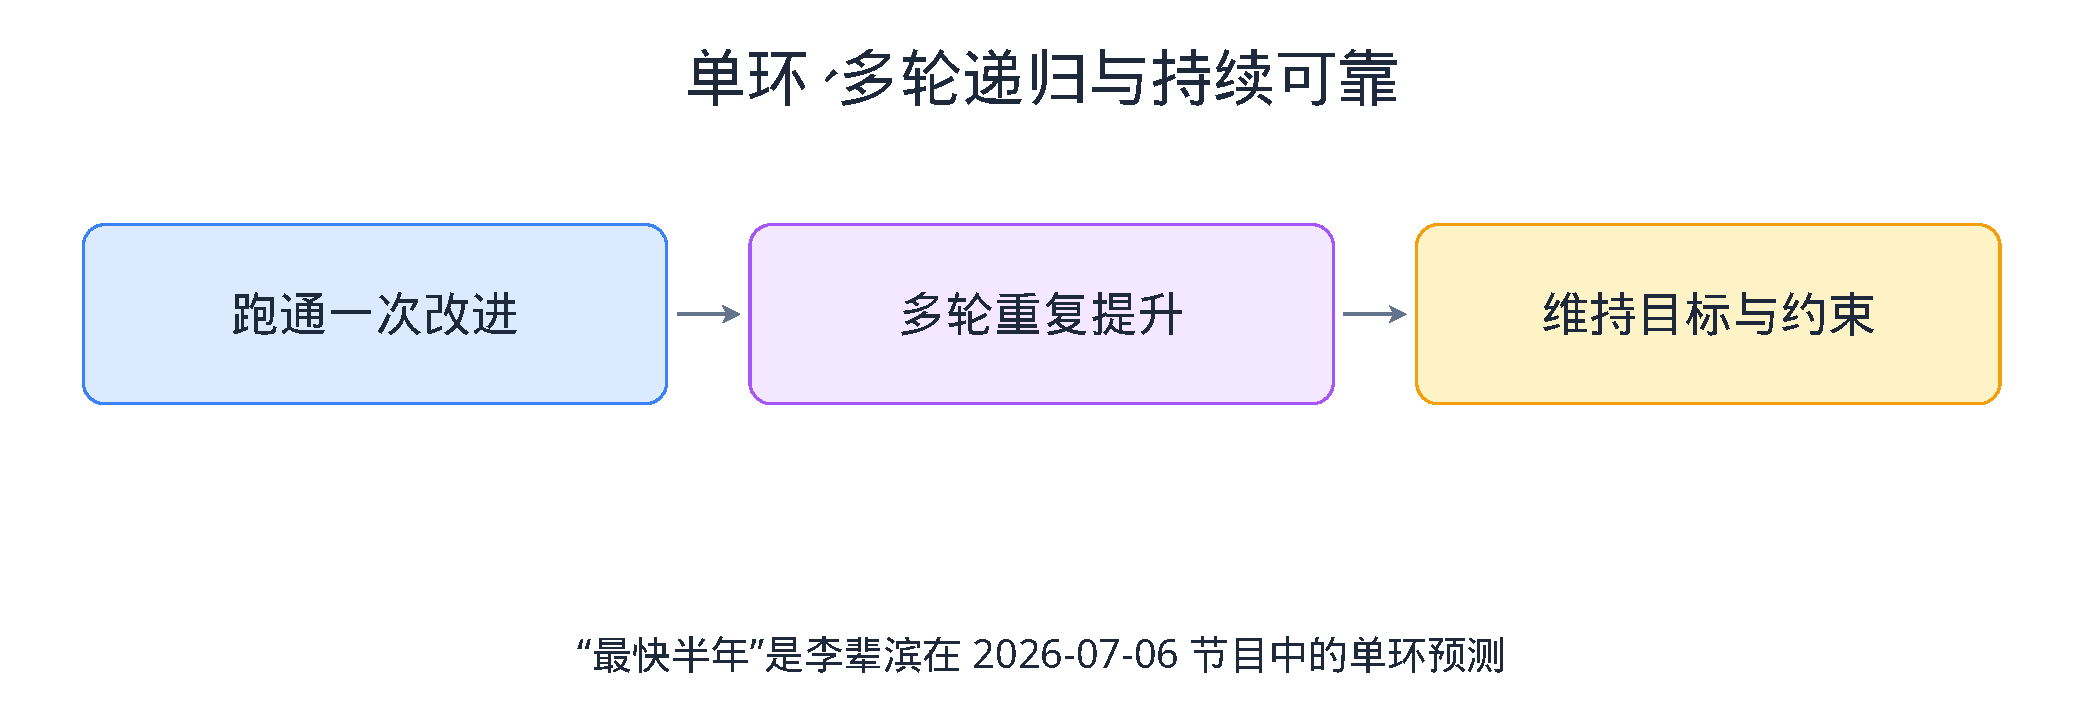
\includegraphics[width=\linewidth,height=.68\textheight,keepaspectratio]{assets/progress-stages.pdf}
\caption{单环、多轮递归与持续可靠（来源：57:53–01:05:04，依据口述整理）}
\end{figure}
\begin{knowledgebox}{读图：半年预测之后仍需回答的问题}
图中自左向右排列三个递进节点：“跑通一次改进”\ensuremath{\rightarrow}“多轮重复提升”\ensuremath{\rightarrow}“维持目标与约束”，底部注明“‘最快半年’是李辈滨在 2026-07-06 节目中的单环预测”。这三个节点分别对应跑通单次后训练闭环（SI）、跨多轮迭代抑制递归漂移，以及在长期迭代中监控未观测维度与安全边界的不同阶段。
\end{knowledgebox}
把单次闭环、多轮递归与目标约束放在同一张路线图上，有助于在总结全篇时客观评估自进化的技术进展与研究判断。
\needspace{6\baselineskip}\subsection{本章小结}
在 2026-07-06 发布的访谈中，李辈滨预计最快半年到一年有望跑通后训练阶段的单次自我提升闭环（SI），而要实现多轮连续递归（RSI），按他的判断仍需再花数年时间压低递归漂移并解决未观测维度的目标妥协问题。在全自动化之前，研究员每天人工阅读智能体操作轨迹、及时停机手调仍是保持可控的重要做法。随着研究者的日常工作从手写代码转向高层监控与品味热启动，节目最后也留下了关于少数人塑造的 AI 品味与普罗大众价值观之间如何对齐的思考。
\needspace{.8\textheight}\section{总结与延伸}
纵观AI自我改进的技术链路，单步解题与连续自进化之间隔着长程执行、可靠验证与品味对齐三道门槛。在系统层面，长程任务需要模型架构优化、长序列训练分布与外部记忆、多智能体分工相互配合；在训练层面，后训练与脚手架如同跑步时的左右脚，当模型的数据分布或行为特点发生改变后，应当重新检查并调整脚手架的匹配方式。为了抑制递归漂移，代码任务依赖边界合理的单元测试，数学推理可引入Lean形式化验证，而缺乏单一规则的开放问题则可采用求解与验证分离的多智能体分工、信源可靠性分级或裁判同步训练等方式来提升验证质量。

按照李辈滨在2026年7月访谈中的判断，最快半年到一年有望跑通的是后训练阶段的单次闭环（SI），即在特定领域完成自我诊断、构造数据、训练与验证提升的一轮循环；要实现多轮连续的递归自我提升（RSI），仍需花更长时间压低每轮迭代的漂移率，并防范模型为迎合显性指标而牺牲成本或其他材料性能。在此之前，人工阅读智能体操作轨迹、及时叫停纠偏仍是日常研发的重要手段。

当工程师的工作重心从逐行手写代码转向高层调度与品味把控，技术演进也把一个更深层的问题推到台前：如果今天AI的科研品味是由极少数顶尖科学家与创始人通过偏好数据和模型宪法来完成热启动的，那么当未来的AI走向更广泛的社会生活时，那些面向普罗大众的应用究竟应该代表谁的价值观？跑通训练闭环只是技术起点，关于价值选择的公共讨论才刚刚开始。
\subsection{拓展阅读}
以下资料供回看节目、查阅术语与继续学习。
\begin{itemize}
\item 硅谷101：本期完整节目：\url{https://www.bilibili.com/video/BV1sAT16WEYg/}
\item Karpathy autoresearch：训练实验的自动迭代：\url{https://github.com/karpathy/autoresearch}
\item Google DeepMind OPRO：语言模型作为优化器：\url{https://github.com/google-deepmind/opro}
\end{itemize}
\end{document}
